\documentclass{beamer}

\usepackage[spanish]{babel}
\usepackage[utf8]{inputenc}
\usepackage[T1]{fontenc}
\usepackage{amsmath,amssymb,amsfonts}
\usepackage{xcolor}
\usepackage{ragged2e}
\usepackage{etoolbox}
\usepackage{lipsum}
\usepackage{csquotes}
\usepackage[center]{caption}
\usepackage[export]{adjustbox}
\usepackage[backend=biber]{biblatex}

\graphicspath{{../Imágenes}}
\addbibresource{../Latex/TFG.bib}

\usetheme{Madrid}
\title[Modelo de Hubbard]{El modelo de Hubbard en materia condensada} 
\author{Luis Lucas García}
\institute[UA]{Universidad de Alicante - Facultad de Ciencias - Grado en física - Trabajo de fin de grado}
\date{Junio de 2025}

\apptocmd{\frame}{}{\justifying}{}
\addtobeamertemplate{block begin}{}{\justifying} % Justify all blocks

\begin{document}
\maketitle
\begin{frame}{Índice}
    \tableofcontents
\end{frame}
\begin{frame}{Segunda cuantización - Operadores de creación y destrucción \cite{LibroQuantum}}
    \section{Fundamentos teóricos}
    \subsection{Segunda cuantización}
    \begin{block}{Operadores de creación y destrucción}
        Se introducen los brakets en notación de segunda cuantización. Introduciendo también la acción de los operadores de creación y destrucción:
        \begin{equation}
            c_i^{\dagger} |\ldots, n_i, \ldots\rangle = (1 - n_i) (-1)^{\sum_{j<i} n_j} | \ldots, n_i + 1, \ldots\rangle
        \end{equation}
        \begin{equation}
            c_i | \ldots, n_i, \ldots\rangle = n_i (-1)^{\sum_{j<i} n_j} | \ldots, n_i, \ldots\rangle
        \end{equation}
    \end{block}
    Bajo la acción de estos operadores, podemos definir cualquier estado a partir del vacío:
    \begin{equation}
        |n_1, n_2, \ldots\rangle = \left( c_1^{\dagger} \right)^{n_1} \left( c_2^{\dagger} \right)^{n_2} \ldots |0\rangle
    \end{equation}
    Y cumplen las siguientes operaciones de conmutación (para fermiones):
    \begin{equation}
        \begin{array}{ccc}
            \left[c_i, c_j\right] = 0 & \left[c_i^{\dagger}, c_j^{\dagger}\right] = 0 & \left[c_i, c_j^{\dagger}\right] = \delta_{ij}
        \end{array}
    \end{equation}
\end{frame}
\begin{frame}{Segunda cuantización - Forma de operadores \cite{LibroQuantum} \cite{Sakurai_Napolitano_2020}}
    \begin{block}{Forma de operadores}
        Estos operadores nos permiten definir la acción de cualquier operador de una o dos partículas de una forma sencilla:
        \begin{align}
            T = \sum_{i, j, \sigma} t_{ij}c_{i, \sigma}^{\dagger}c_{j, \sigma} \\
            F = \frac{1}{2}\sum_{i, j, k, l, \sigma} V_{ijkl}c_{i, \sigma}^{\dagger}c_{j, \sigma}^{\dagger}c_{k, \sigma} c_{l, \sigma}
            \label{eq:sqOperators}
        \end{align}
    \end{block}
    Y los elementos de matriz se calculan como:
    \begin{equation}
        \begin{split}
            t_{ij} = \langle i | \hat{t} | j \rangle = \int d\vec{r} \, \phi_i^*(\vec{r}) \hat{T} \phi_j(\vec{r}) \\ V_{ijkl} = \langle i, j | f^{(2)} | k, l \rangle = \int\int d\vec{r}_1 d\vec{r}_2 \, \phi_i^*(\vec{r}_1) \phi_j^*(\vec{r}_2) \hat{V} \phi_k(\vec{r}_2) \phi_l(\vec{r}_1)
        \end{split}
    \end{equation}
\end{frame}
\begin{frame}{Segunda cuantización - Operadores de campo \cite{LibroQuantum} \cite{Sakurai_Napolitano_2020}}
    Finalmente, introducimos los operadores de campo, para más adelante introducir las funciones de Green. Realicemos un cambio de base al espacio de posiciones usando:
    $$
    |\lambda\rangle = \sum_i |i\rangle\langle i|\lambda\rangle
    $$
    \begin{block}{Operadores de campo}
        Introducimos a continuación los operadores de campo, como los operadores de creación y destrucción que crean o destruyen un autoestado de la posición.
        \begin{equation}
            \begin{array}{cc}
                \psi(\vec{x}) = \sum_i \varphi (\vec{x}) c_i & \psi^{\dagger} (\vec{x}) = \sum_i \varphi_i^* (\vec{x}) c_i^{\dagger}
            \end{array}
        \label{eq:FieldOps}
        \end{equation}
    \end{block}
    Y cumplen unas relaciones de conmutación similares:
    \begin{align*}
        \begin{array}{cc}
            [\psi(\vec{x}), \psi(\vec{x}')]_{\pm} = 0 & [\psi^{\dagger}(\vec{x}), \psi^{\dagger}(\vec{x}')]_{\pm} = 0
            \end{array} \\
        \begin{array}{c}
        [\psi(\vec{x}), \psi^{\dagger}(\vec{x}')]_{\pm} = \delta^{(3)} (\vec{x} - \vec{x}')
    \end{array}
    \end{align*}
\end{frame}
\begin{frame}{Modelo de tight-binding \cite{AshcroftSSP} \cite{simon2013oxford}}
    \subsection{Modelo de tight-binding}
    \begin{figure}[h!]
        \begin{center}
            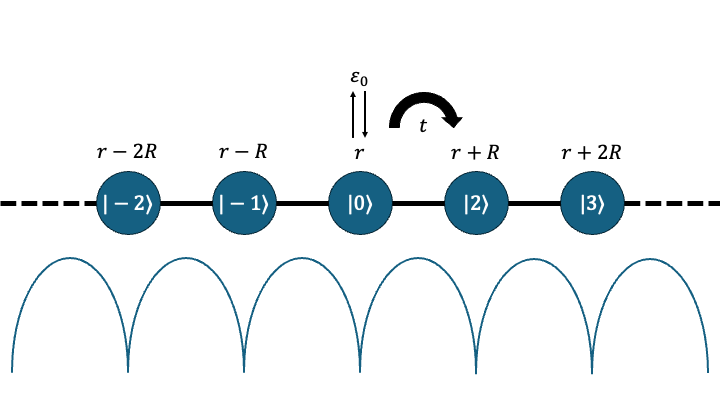
\includegraphics[max width=0.85\linewidth]{AtomicChain.png}
            \caption{Cadena de átomos, donde los círculos representan los núcleos. En cada átomo podemos ubicar dos electrones, uno con cada spin, y pueden saltar de un elemento a otro por el término de hopping.}
            \label{fig:TBChain}
        \end{center}
    \end{figure}
\end{frame}
\begin{frame}
    La solución la escribimos como combinación lineal de orbitales atómicos. El hamiltoniano de tight-binding tendrá la forma:
    \begin{equation}
        \sum_m H_{nm}\phi_m = E\phi_n
    \end{equation}
    Donde se cumple que:
    \begin{equation}
        H_{nm} = \varepsilon_0\delta_{nm} + \sum_{n\neq m}\langle n | V | m \rangle
    \label{eq:hamElements}
    \end{equation}
    Donde $\langle n | V | m \rangle$ serán los elementos de hopping, que si lo tomamos a primeros vecinos:
    \begin{equation}
        t_{xy} = \left\{\begin{array}{cc}
            t, & |x - y| = 1 \\
            0, & \text{en otro caso}
        \end{array}\right.
        \label{eq:hoppinFN}
    \end{equation}
    Vamos a tomar condiciones periódicas. Usando una solución que cumpla el teorema de Bloch, $\phi_n = \frac{e^{-ikna}}{\sqrt{N}}$ ,tendremos la ecuación de las bandas:
    \begin{equation}
        E = \varepsilon_0 - 2tcos(ka)
        \label{eq:bandasTB}
    \end{equation}
\end{frame}
\begin{frame}
    \begin{figure}[h!]
        \begin{center}
            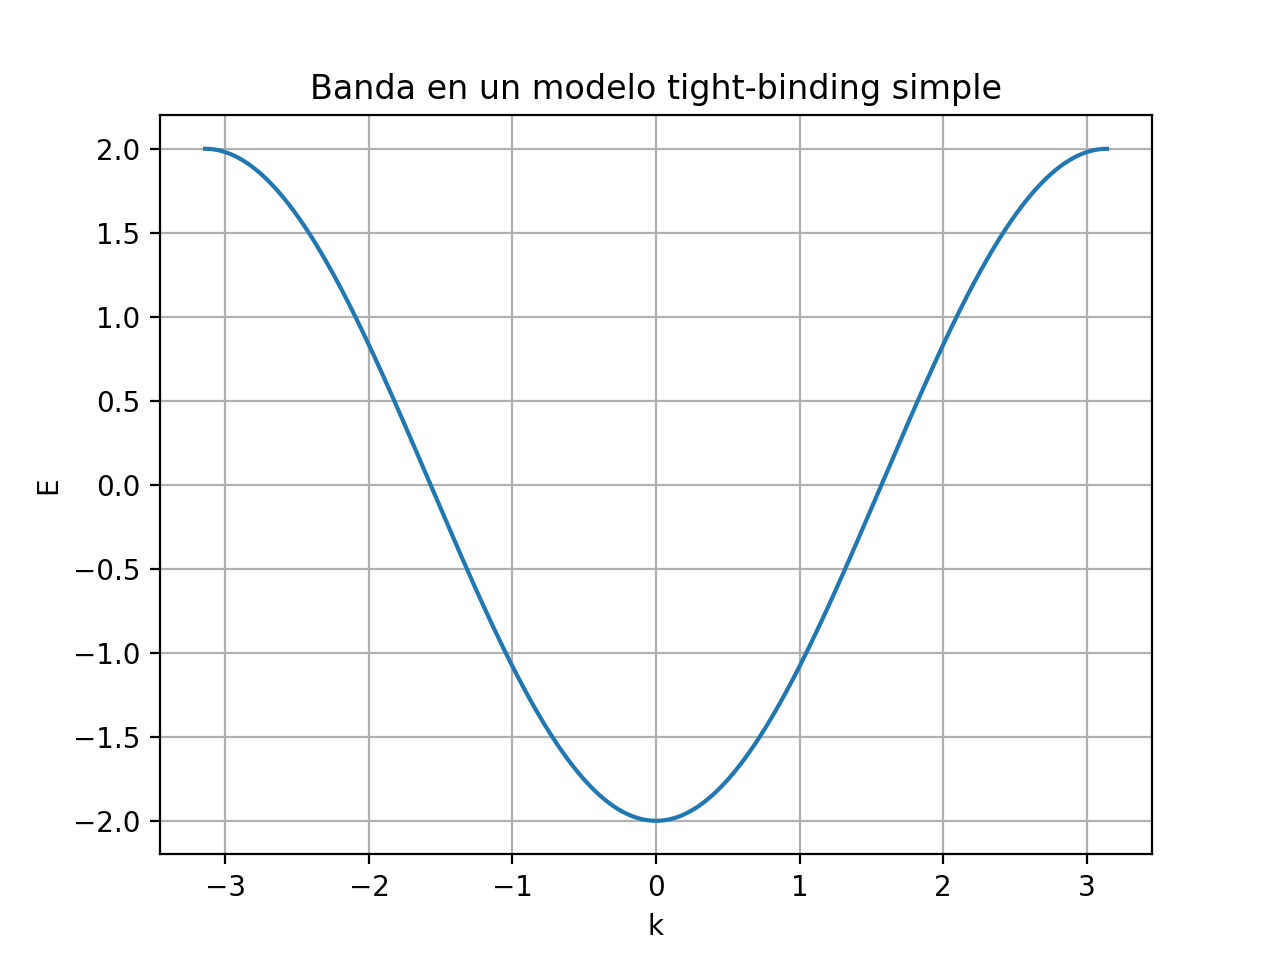
\includegraphics[max width=0.8\linewidth]{BandTB.png}
            \caption{La única banda que aparece en el sistema de tight-binding que hemos considerado. Estamos considerando $\varepsilon_0 = 0$ y $t = 1$.}
            \label{fig:bandaTB}
        \end{center}
    \end{figure}
\end{frame}
\begin{frame}
    \begin{block}{Densidad de estados}
        Vamos a definir a continuación la densidad de estados (en inglés la DOS). Es una función que define la probabilidad de encontrar una partícula a una energía dada, y se construye siguiendo la expresión:
        \begin{equation}
            N = \int_0^{E_F} g(E) \, dE
        \end{equation}
    \end{block}
    Además, en esta definición ya aparece otra cantidad importante, que es la energía de Fermi. Representa una energía a la que, si integramos nuestra densidad de estados, deben de aparecer todos los electrones del sistema, es decir, todos los niveles de energía por debajo de la energía de Fermi están ocupados y por encima desocupados.

    La densidad de estados para el sistema que estamos estudiando es:
    \begin{equation}
        g(E) = \frac{1}{\pi at}\frac{1}{\sqrt{1-\left(\frac{E}{2t}\right)^2}}
    \end{equation}
\end{frame}
\begin{frame}
    \begin{figure}[h!]
        \begin{center}
            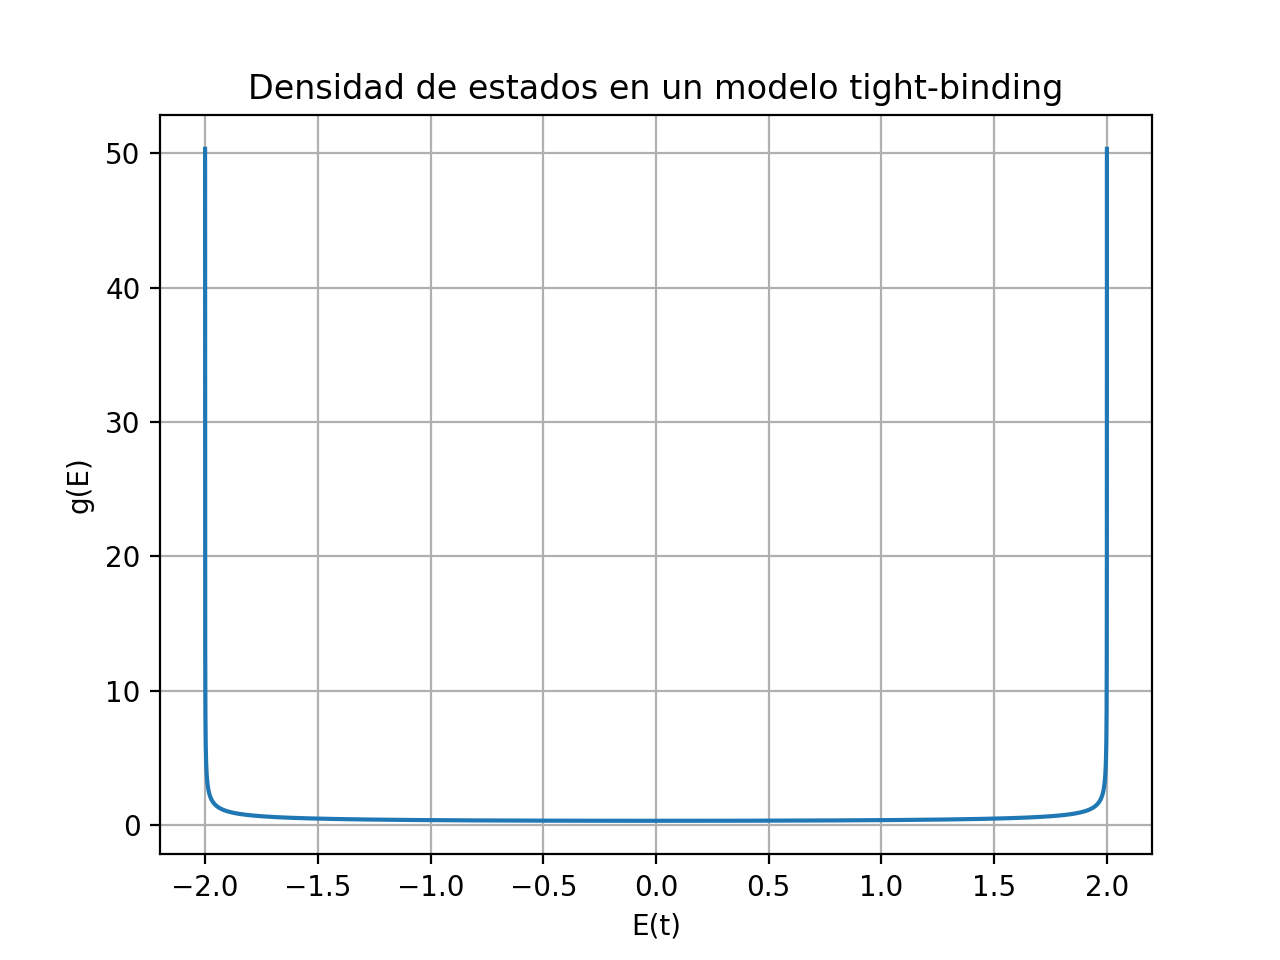
\includegraphics[max width=0.7\linewidth]{DosTB.png}
            \caption{Densidad de estados en un modelo sencillo de tight-binding. Se puede observar el efecto de las singularidades de Van-Hove. En este caso, nuestra energía de Fermi está en $E_F = 0$, situándose en el centro y los fermiones se ubican en los niveles más bajos de energía. Nuevamente consideramos $\varepsilon_0 = 0$ y $t = 1$.}
            \label{fig:dosTB}
        \end{center}
    \end{figure}
\end{frame}
\begin{frame}{El modelo de Hubbard \cite{MielkeHubbard}}
    \subsection{El modelo de Hubbard}
    \begin{block}{Hamiltoniano de Hubbard}
        Podemos escribir el hamiltoniano de Hubbard en segunda cuantización con lo que hemos visto:
        \begin{equation}
            H = \sum_{x, y, \sigma}t_{xy}c^{\dagger}_{x,\sigma}c_{y,\sigma} + \sum_x U_x c^{\dagger}_{x\uparrow}c^{\dagger}_{x\downarrow}c_{x\downarrow}c_{x\uparrow}
        \end{equation}
    \end{block}
    Este hamiltoniano cumple algunos teoremas interesantes que aparecen en el artículo \cite{MielkeHubbard}. Cito a continuación algunos:
    \begin{enumerate}
        \item \textbf{Teorema de Lieb, 1989:} el hamiltoniano de Hubbard con $U_x < 0$, con un número de partículas par, presenta un único estado fundamental, de spin total $S = 0$.
        \item \textbf{Corolario:} El hamiltoniano de Hubbard, con interacción $U_x > 0$ y un número de partículas con semillenado, el estado fundamental es único en el subespacio $S_z = 0$ con spin total $S = \frac{1}{2}\left||A| - |B|\right|$.
    \end{enumerate}
\end{frame}
\begin{frame}{Funciones de Green \cite{fetter1971quantum}}
    \subsection{Funciones de Green}
    \begin{block}{Funciones de Green}
        Se introduce la función de Green como:
        \begin{equation}
            iG_{\alpha\beta}(\vec{x}t, \vec{x}'t') = \frac{\left\langle\Psi_0|T\left(\hat{\psi}_{H\alpha}(\vec{x}t)\hat{\psi}^{\dagger}_{H\beta}(\vec{x}'t')\right)|\Psi_0\right\rangle}{\langle\Psi_0|\Psi_0\rangle}
            \label{eq:GreenFunction}
        \end{equation}
    \end{block}
    En la expresión anterior, $T$ es el operador de ordenación temporal y $\hat{\psi}_{H\alpha}$ es el operador de campo en la representación de Heisenberg. El operador temporal actúa tal que:
    \begin{equation}
        T\left(\hat{\psi}_{H\alpha}(\vec{x}t)\hat{\psi}^{\dagger}_{H\beta}(\vec{x}'t')\right) = \left\{\begin{array}{cc}
        \hat{\psi}_{H\alpha}(\vec{x}t)\hat{\psi}^{\dagger}_{H\beta}(\vec{x}'t') & t > t' \\
        \pm\hat{\psi}_{H\alpha}^{\dagger}(\vec{x}'t')\hat{\psi}_{H\beta}(\vec{x}t) & t' > t
        \end{array}\right.
    \end{equation}
    Donde, en la segunda ocasión ocurre el cambio de signo para el caso de fermiones. Usando el anticonmutador de los operadores de campo, podemos definir las funciones de Green avanzada y retardada.
\end{frame}
\begin{frame}{Funciones de Green - Aplicaciones \cite{fetter1971quantum}}
    La aplicación más importante de las funciones de Green para este trabajo es la del cálculo de la densidad de estados. Introducimos las funciones de Green en la representación $\omega$-Lehman.
    \begin{equation}
        \begin{array}{cc}
            \hat{G}^+(\omega) = \lim_{\eta\to 0^+}\frac{1}{\omega - H + E_0 + i\eta} & \hat{G}^-(\omega) = \lim_{\eta\to 0^+}\frac{1}{\omega + H - E_0 - i\eta}
        \end{array}
    \end{equation}
    \begin{block}{Densidad de estados}
        Con las funciones de Green en esta representación podemos conseguir la densidad de estados.
        \begin{equation}
            \begin{split}
                Im(G^+(\vec{R}, \vec{R}, \omega)) = -\pi\frac{1}{V}\sum_{\vec{k}, \varepsilon_{\vec{k}}\gtrless\varepsilon_F}\delta(\omega - \varepsilon_{\vec{k}}) = -\pi DOS(\omega) \implies \\ -\frac{1}{\pi}Im\left(G^+\left(\vec{R}, \vec{R}, \omega\right)\right) = DOS\left(\omega\right)
            \end{split}
        \end{equation}
    \end{block}
\end{frame}
\begin{frame}{El algoritmo de Lanczos \cite{RevModPhys.66.763} \cite{GreeneDiniz2024}}
    \section{El algoritmo de Lanczos}
    El algoritmo de Lanczos nos permite obtener una base en la que un hamiltoniano se representa como matriz tridiagonal. El problema es la alta dimensionalidad del espacio en el modelo de Hubbard.
    $$
    dimn = \left(\begin{array}{c}
    N \\
    N_{\uparrow}
    \end{array}\right)\left(\begin{array}{c}
    N \\
    N_{\downarrow}
    \end{array}\right)
    $$
    \begin{block}{Descripción del método}
        En el algoritmo de Lanczos, se calculan los elementos de la base tal que:
        \begin{equation}
            \begin{array}{cc}
                a_n = \frac{\langle\phi_n|\hat{H}|\phi_n\rangle}{\langle\phi_n|\phi_n\rangle} & b_n^2 = \frac{\langle\phi_n|\phi_n\rangle}{\langle\phi_{n-1}|\phi_{n-1}\rangle}
            \end{array}
    \end{equation}
    \begin{equation}
        |\phi_{n+1}\rangle = \hat{H}|\phi_n\rangle - a_n|\phi_n\rangle - b_n^2|\phi_{n-1}\rangle
    \end{equation}
    Donde además, tenemos que dotar de la condición $b_0 = 0$.
    \end{block}
\end{frame}
\begin{frame}
    \begin{equation}
        H = \left(\begin{array}{ccccc}
            a_0 & b_1 & 0 & 0 & \ldots \\
            b_1 & a_1 & b_2 & 0 & \ldots \\
            0 & b_2 & a_2 & b_3 & \ldots \\
            0 & 0 & b_3 & a_3 & \ldots \\
            \vdots & \vdots & \vdots & \vdots & \ddots
        \end{array}\right)
    \end{equation}
    \subsection{Algoritmo modificado}
    Puesto que el algoritmo de Lanczos converge bastante rápido al estado fundamental, podemos aprovecharlo para usarlo de modo iterativo con unos pocos pasos. El procedimiento es:
    \begin{enumerate}
        \item Tomar un vector, $\phi_0$, inicial arbitrario.
        \item Aplicar un número $l$ de iteraciones de Lanczos y obtener el autovalor mínimo del hamiltoniano $l \times l$, $E_0$, y su autovector correspondiente, $\psi_0$.
        \item Obtenemos un nuevo vector inicial, $\psi_0$. Si la energía cumple la condición de convergencia, tenemos nuestro estado fundamental y energía. Si no, almacenamos en memoria $E_0$ y repetimos el paso 2 pero con el nuevo vector $\psi_0$ como vector inicial.
    \end{enumerate}
\end{frame}
\begin{frame}{Función de Green de una partícula \cite{RevModPhys.66.763} \cite{GreeneDiniz2024}}
    \subsection{Funciones de Green}
    Para calcular la función de Green necesitamos volver a ejecutar el algoritmo de Lanczos, una vez por cada parte (partículas y huecos), pero con unos estados iniciales modificados.
    \begin{equation}
        \begin{array}{cc}
            \left|\psi_{i, i}^{(h)}\right\rangle = \frac{c_{i\sigma}^{\dagger}\left|\psi_0\right\rangle}{\sqrt{n_{i, i}^{(p)}}} & \left|\psi_{i, i}^{(p)}\right\rangle = \frac{c_{i\sigma}\left|\psi_0\right\rangle}{\sqrt{n_{i, i}^{(h)}}} \\ n_{i, i}^{(p)} = \left\langle\psi_0\left| c_{i\sigma}^{\dagger}c_{i\sigma}\right|\psi_0\right\rangle & n_{i, i}^{(h)} = \left\langle\psi_0\left| c_{i\sigma}c_{i\sigma}^{\dagger}\right|\psi_0\right\rangle
        \end{array}
    \end{equation}
    \begin{figure}
        \begin{center}
            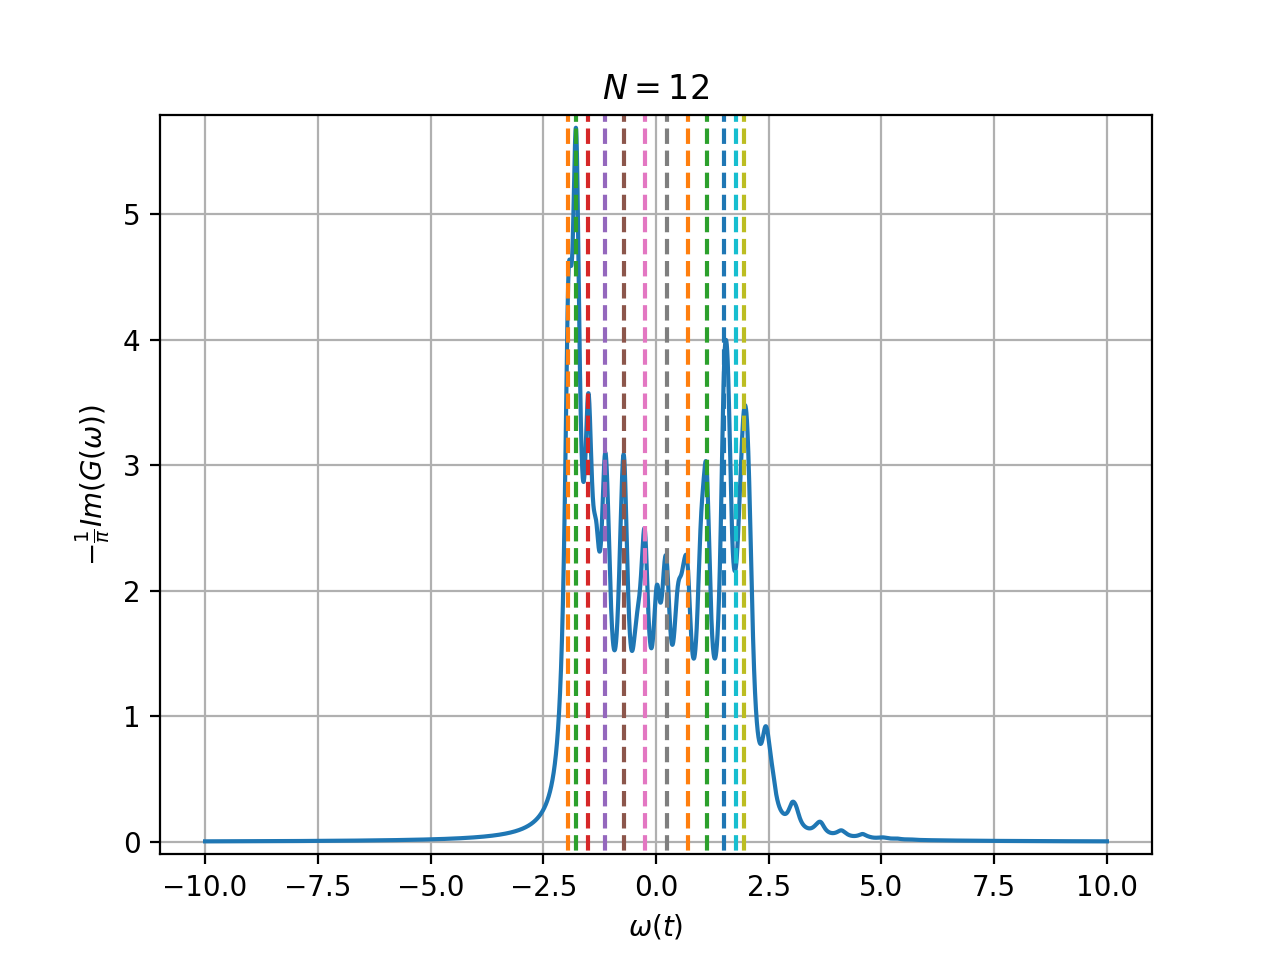
\includegraphics[max width=0.29\linewidth]{lanczosTB12.png}
            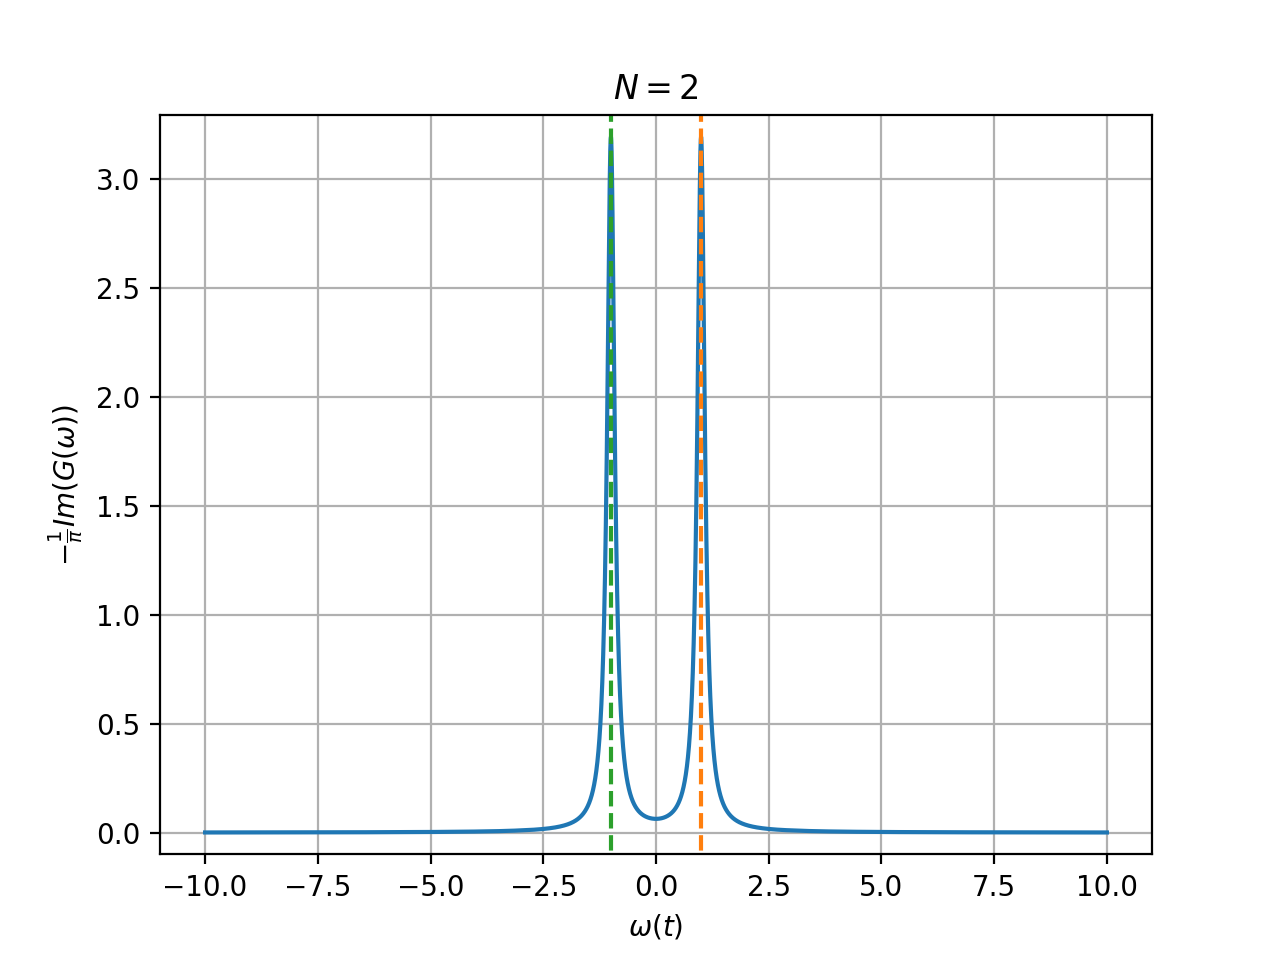
\includegraphics[max width=0.29\linewidth]{lanczosTB2.png}
            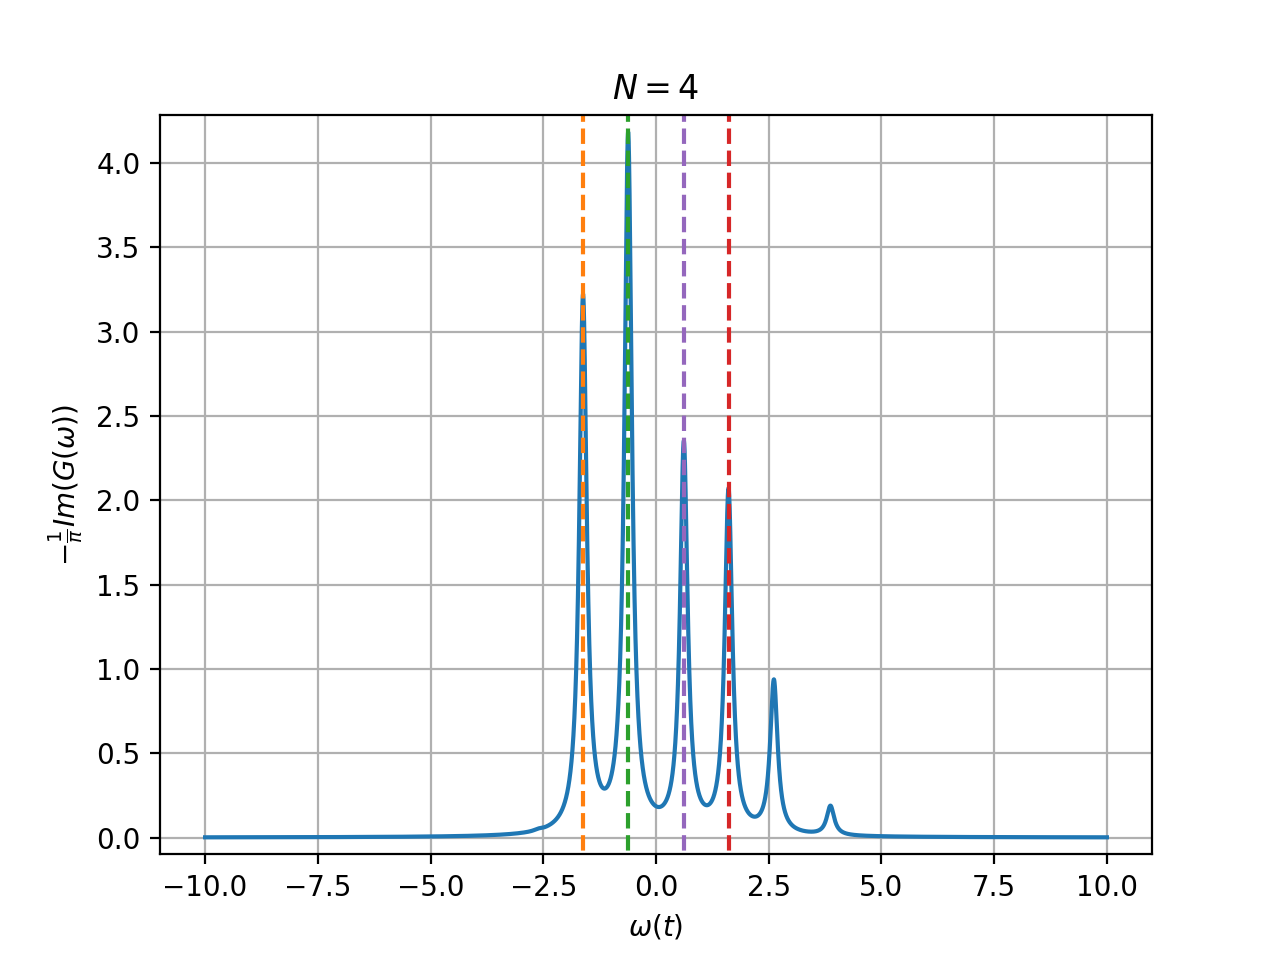
\includegraphics[max width=0.29\linewidth]{lanczosTB4.png}
        \end{center}
        \caption{Funciones de Green del modelo de tight-binding convergidas por el algoritmo de Lanczos.}
    \end{figure}
\end{frame}
\begin{frame}
    \begin{block}{Función de Green}
        \begin{equation}
            \begin{split}
                G_{i, i} = \frac{n_{i, i}^{(h)}}{\omega + E_0 - a_0^{(h)} - \frac{\left(b_1^{(h)}\right)^2}{\omega + E_0 - a_1^{(h)} - \frac{\left(b_2^{(h)}\right)}{\omega + E_0 - a_2^{(h)} - \ldots}}} + \\ + \frac{n_{i, i}^{(p)}}{\omega - E_0 + a_0^{(p)} - \frac{\left(b_1^{(p)}\right)^2}{\omega - E_0 + a_1^{(p)} - \frac{\left(b_2^{(p)}\right)}{\omega - E_0 + a_2^{(p)} - \ldots}}}
            \end{split}
            \label{eq:greenLanczos}
        \end{equation}
    \end{block}
    \begin{figure}
        \begin{center}
            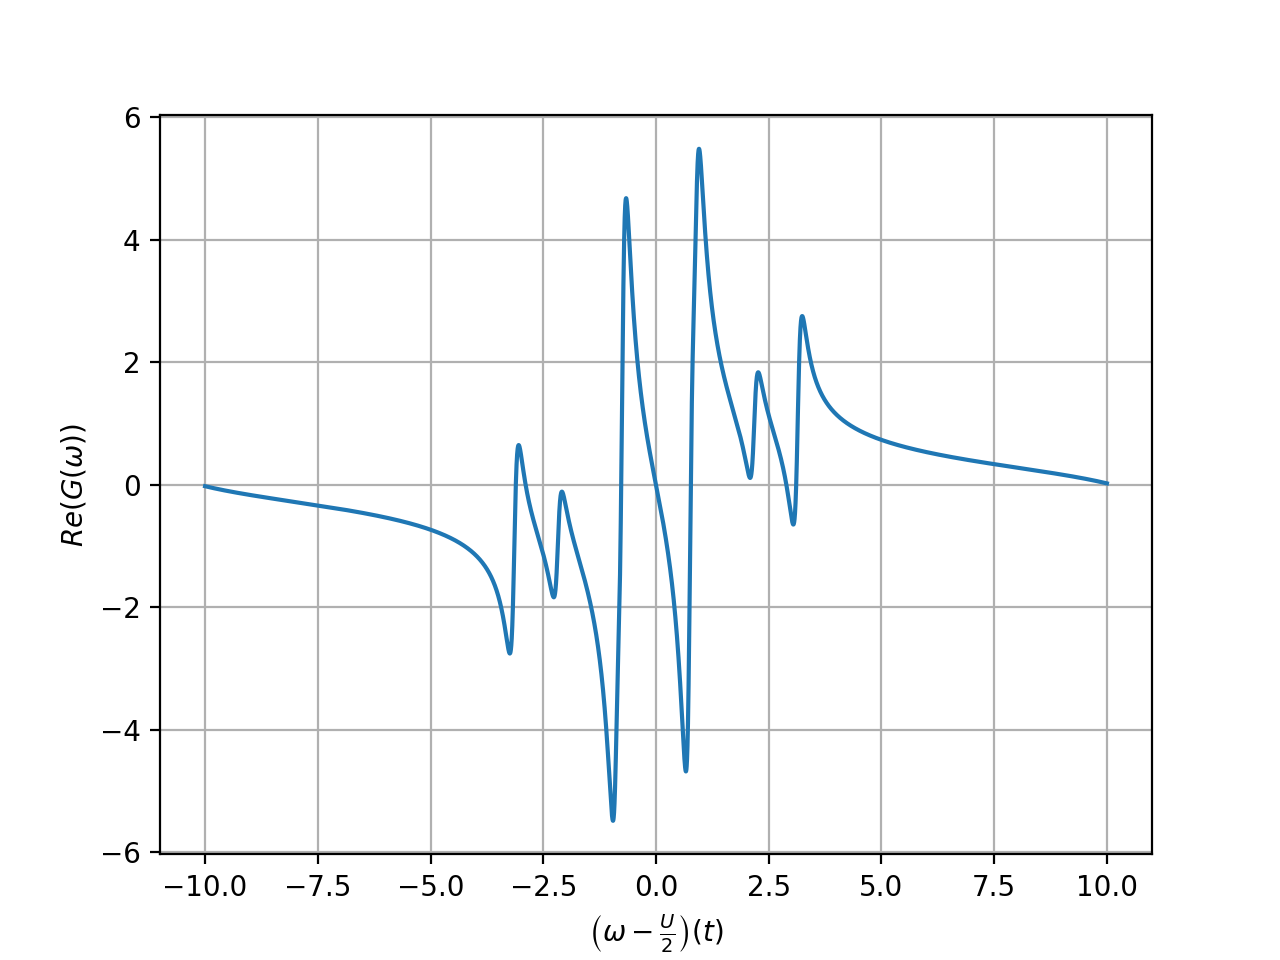
\includegraphics[max width=0.19\linewidth]{lanczosHubbard6U2Real.png}
            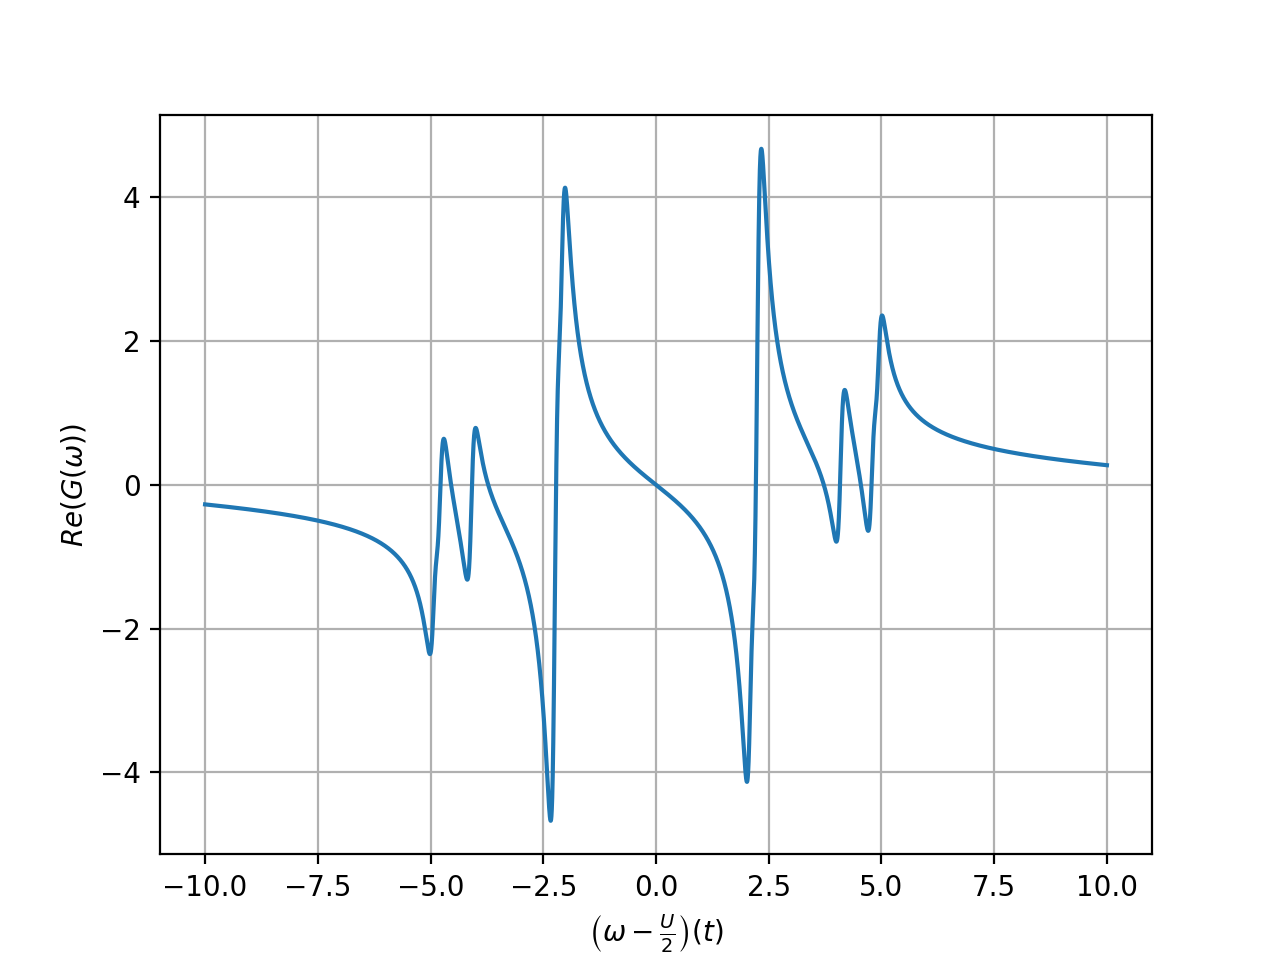
\includegraphics[max width=0.19\linewidth]{lanczosHubbard6U6Real.png}
            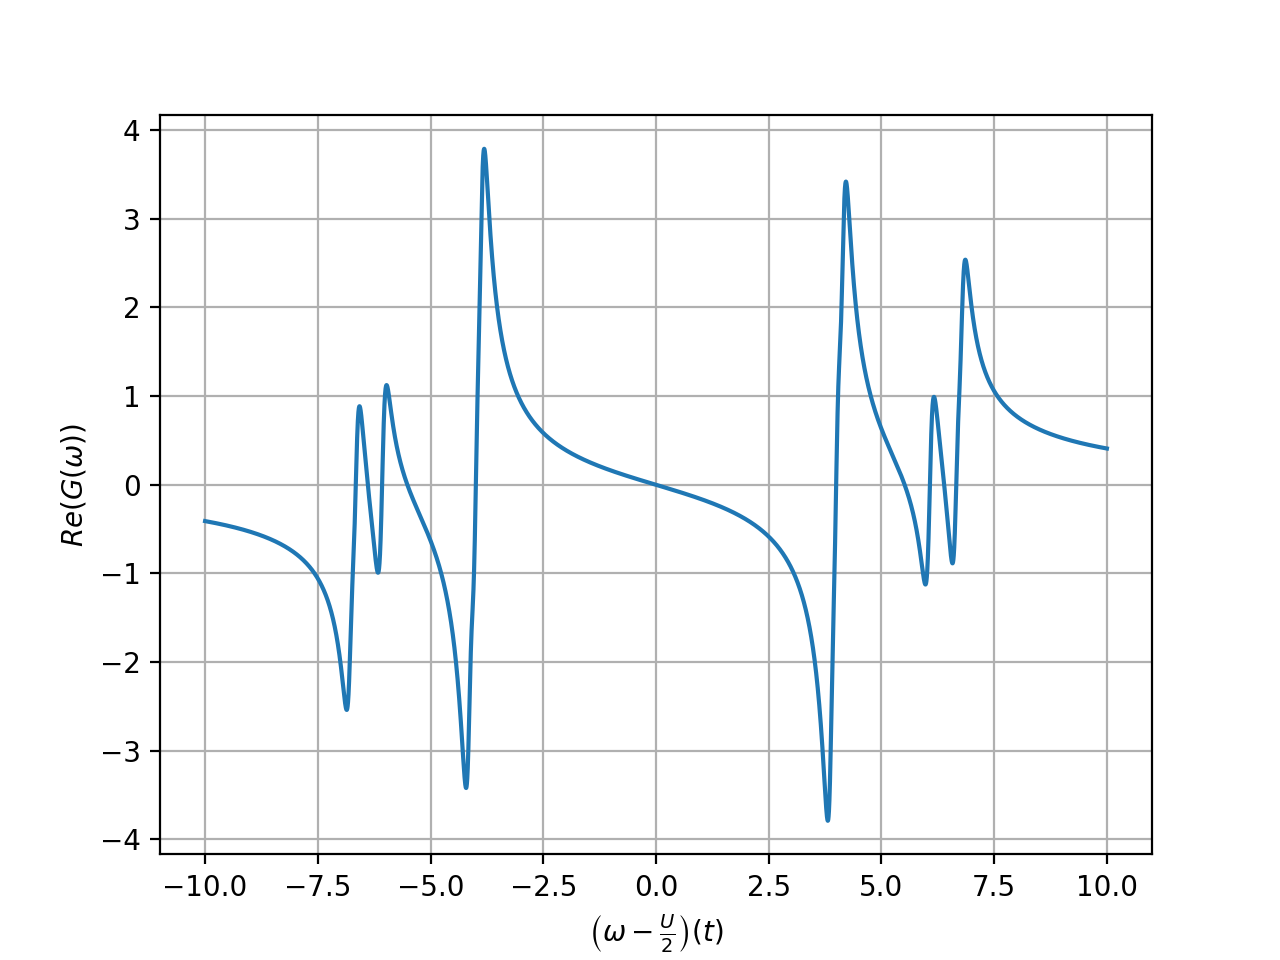
\includegraphics[max width=0.19\linewidth]{lanczosHubbard6U10Real.png}
        \end{center}
        \caption{Partes reales de algunas funciones de Green del modelo de Hubbard.}
    \end{figure}
\end{frame}
\begin{frame}{Desarrollo - Tratamiento de datos}
    \section{Desarrollo}
    \subsection{Tratamiento de datos}
    Para representar la función de onda, vamos a representar los electrones con spin up y spin down como una cadena binaria cada una, y esa cadena binaria, como un número decimal, para ocupar menos espacio.
    $$
    \begin{array}{cc}
        |\psi_{i\uparrow}\rangle = |1, 0, 0, 1, \ldots, 0\rangle = |x\rangle_n & |\psi_{i\downarrow}\rangle = |0, 1, 0, 1, \ldots, 1\rangle = |y\rangle_n
    \end{array}
    $$
    \begin{block}{Función de onda}
        Representaremos la función de onda dentro de nuestro programa como:
        $$
        |\psi\rangle = \sum_i\alpha_i|x_i\rangle_N|y_i\rangle_N
        $$
        De este modo, sólo necesitaremos almacenar tres listas en memoria, una con los coeficientes en float, y dos de enteros, que representarán las cadenas de spin up y spin down.
    \end{block}
\end{frame}
\begin{frame}{Desarrollo - Casos de control}
    \subsection{Casos de control}
    \begin{figure}[h!]
        \begin{center}
            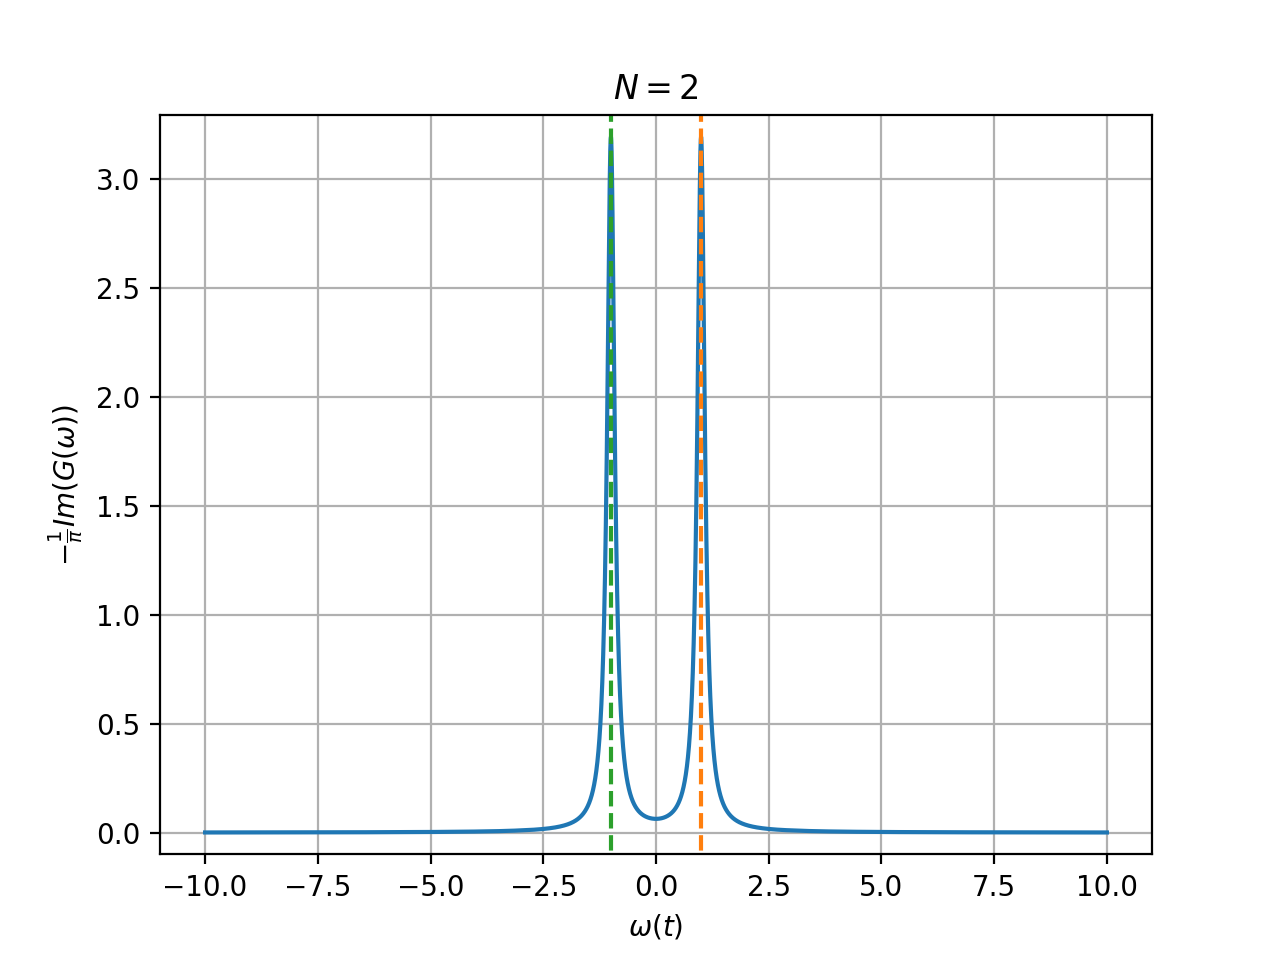
\includegraphics[max width=0.42\linewidth]{lanczosTB2.png}
            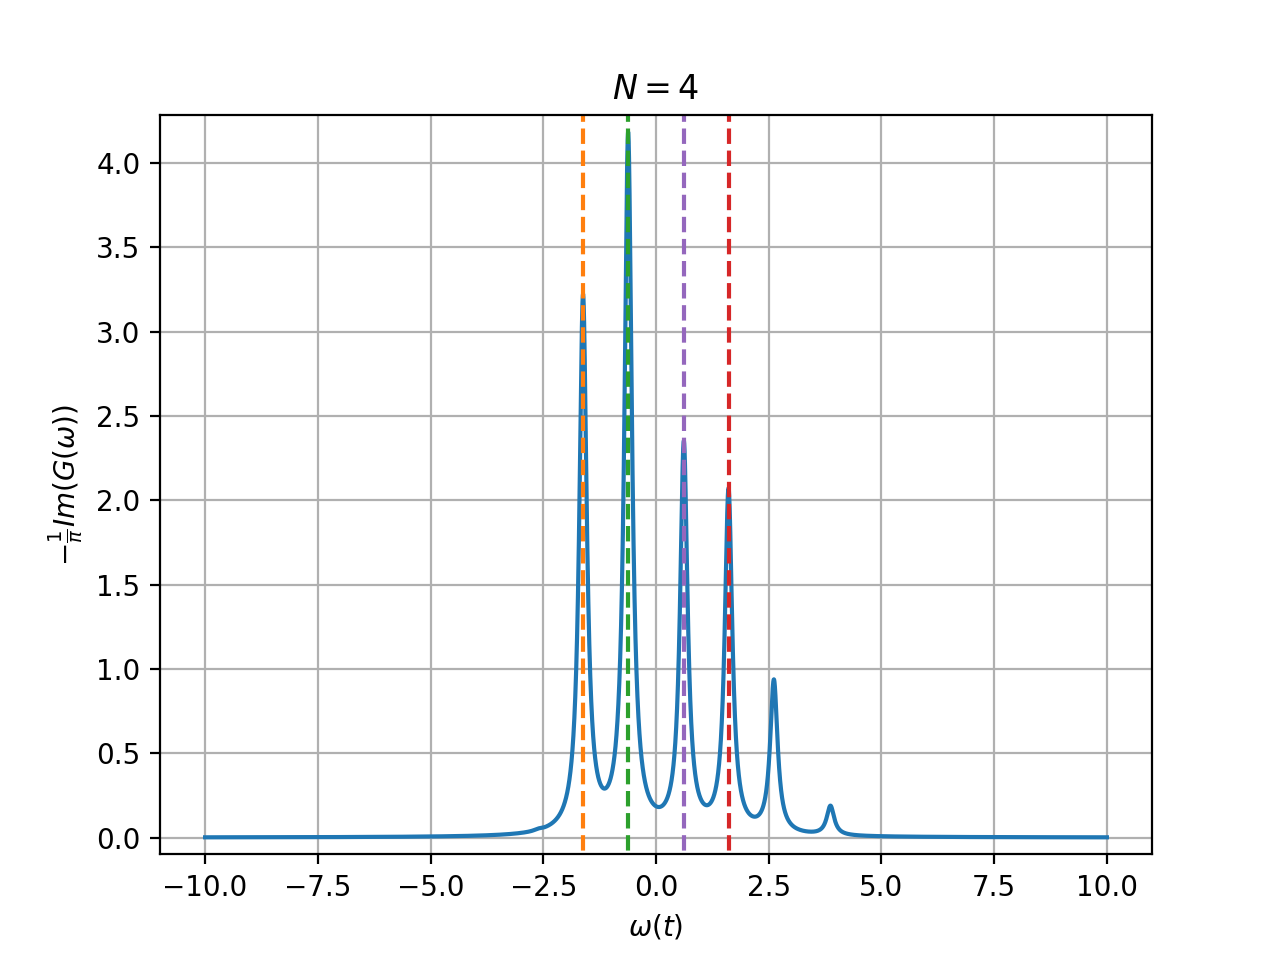
\includegraphics[max width=0.42\linewidth]{lanczosTB4.png}
            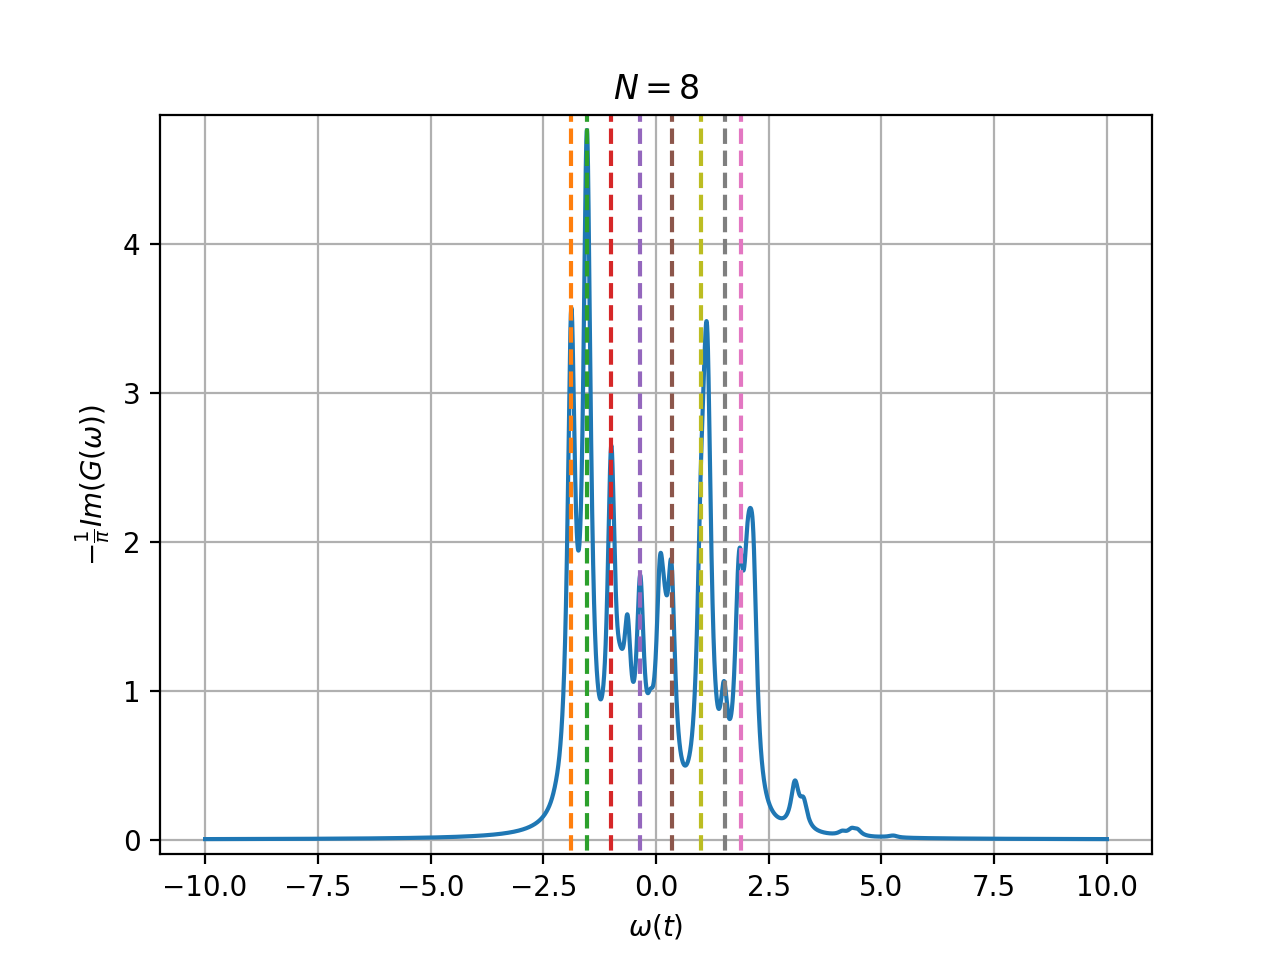
\includegraphics[max width=0.42\linewidth]{lanczosTB8.png}
            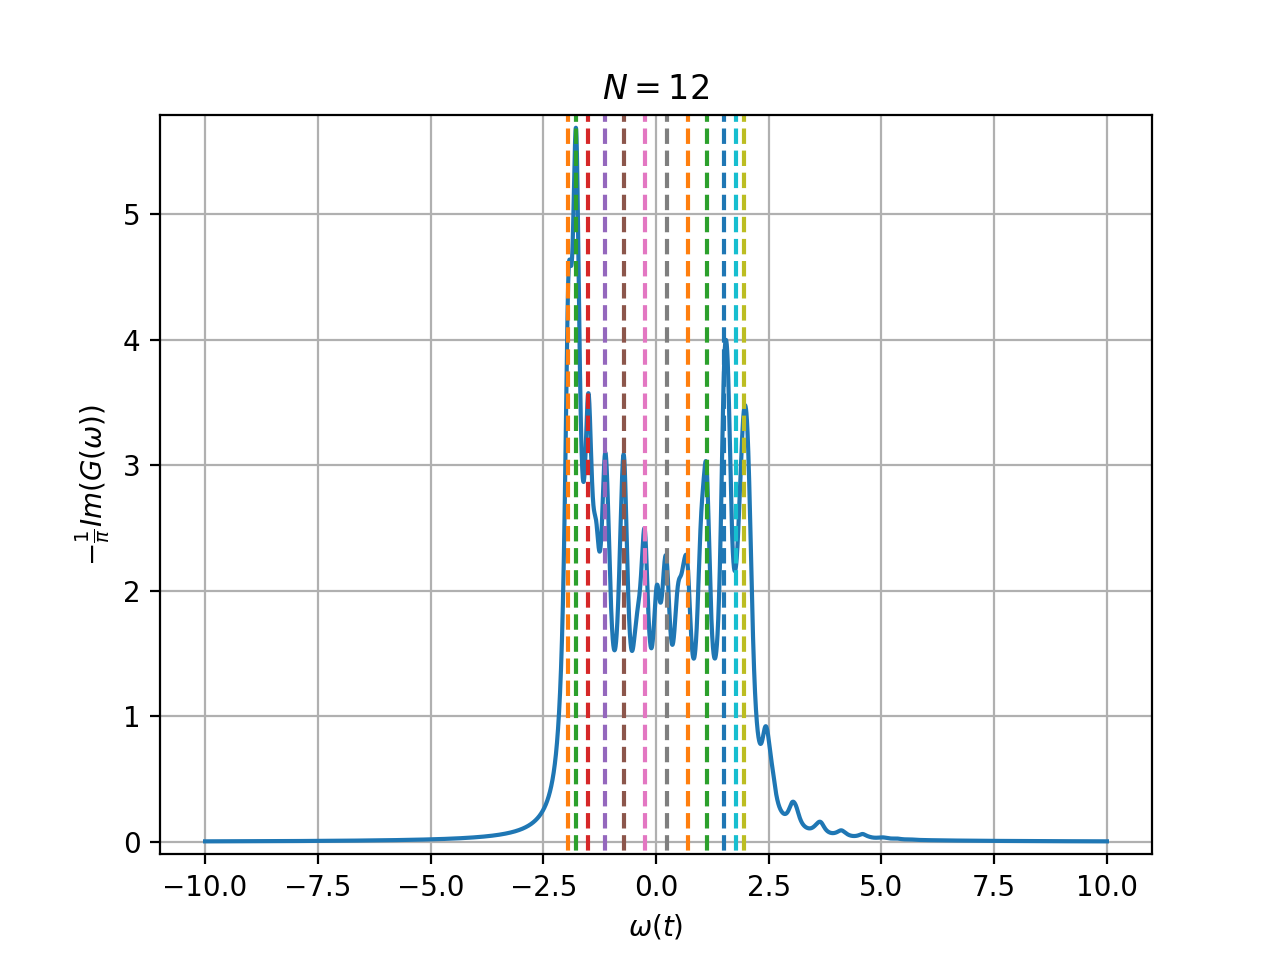
\includegraphics[max width=0.42\linewidth]{lanczosTB12.png}
        \end{center}
        \label{fig:greenTB}
    \end{figure}
\end{frame}
\begin{frame}
    Si observamos la figura \ref{fig:greenTB}, nos podría preocupar que los picos de la densidad de estados no coinciden exactamente, pero vamos a ir viendo que esto es ruido del propio cálculo numérico. Las causas del ruido pueden ser varias:
    \begin{itemize}
        \item \textit{Tolerancia limitada}. Aunque estamos exigiendo como criterio de convergencia una tolerancia de $10^{-6}$, el hecho de estar utilizando una diagonalización iterativa y no exacta puede estar causando ruido.
        \item \textit{Las condiciones de contorno no son periódicas}. Tras haber trabajado bastante con el programa, añadir las condiciones periódicas elimina el ruido en gran medida.
        \item \textit{Faltan funciones de Green}. Como ya hemos mencionado, para calcular la función de Green debemos de hacer dos iteraciones más de Lanczos por cada elemento. Esto es muy costoso en tiempo, por lo que, en vez de hacer las iteraciones con la dimensionalidad completa del espacio de Krylov, tomamos sólo un número limitado de raíces de Lanczos para reducir el tiempo de cómputo.
    \end{itemize}
\end{frame}
\begin{frame}{Desarrollo - Transición metal-aislante}
    \subsection{Transición metal-aislante}
    \begin{figure}
        \begin{center}
            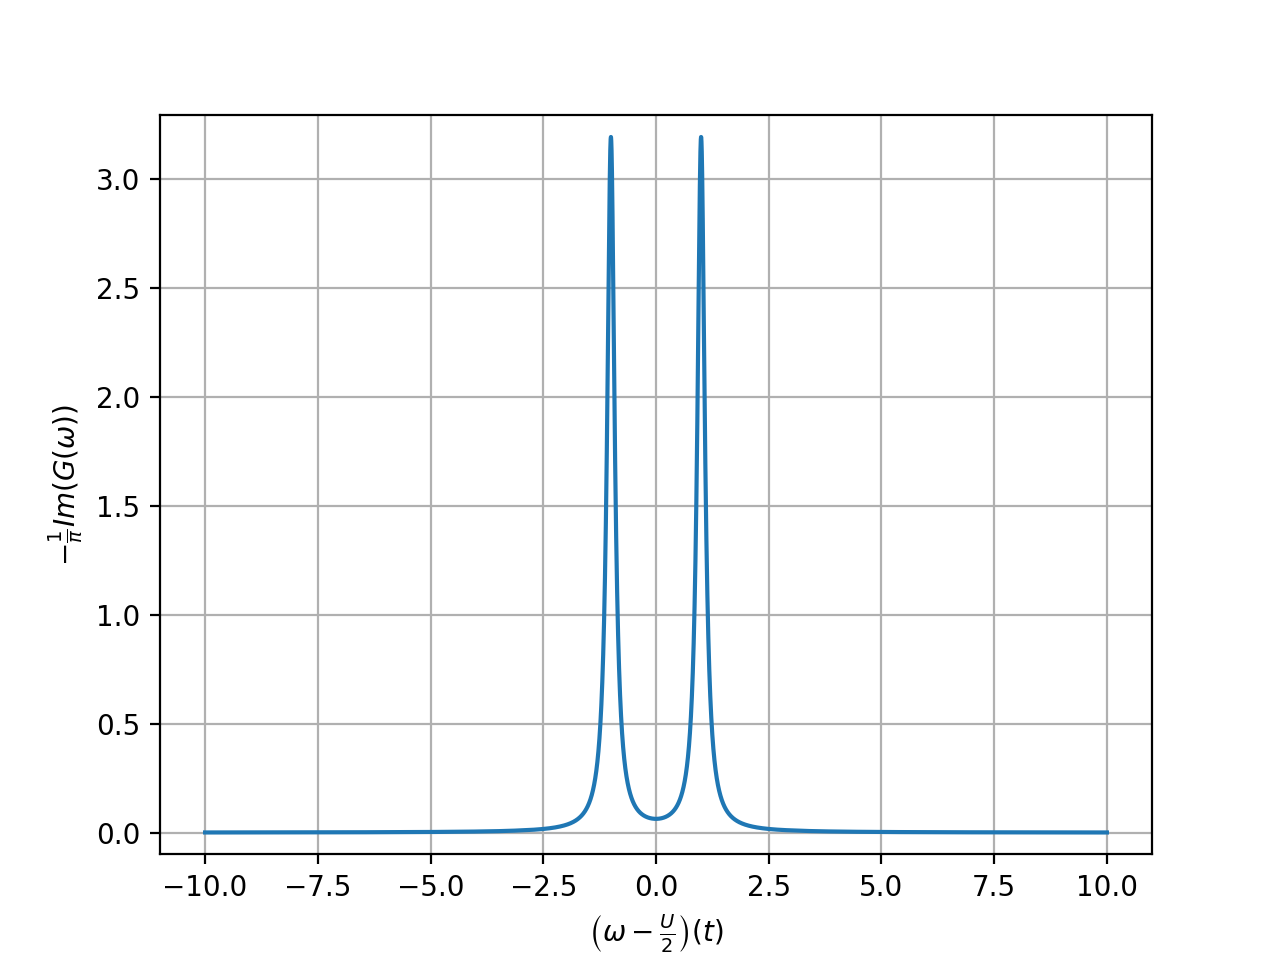
\includegraphics[max width=0.49\linewidth]{lanczosHubbard2U0Imag.png}
            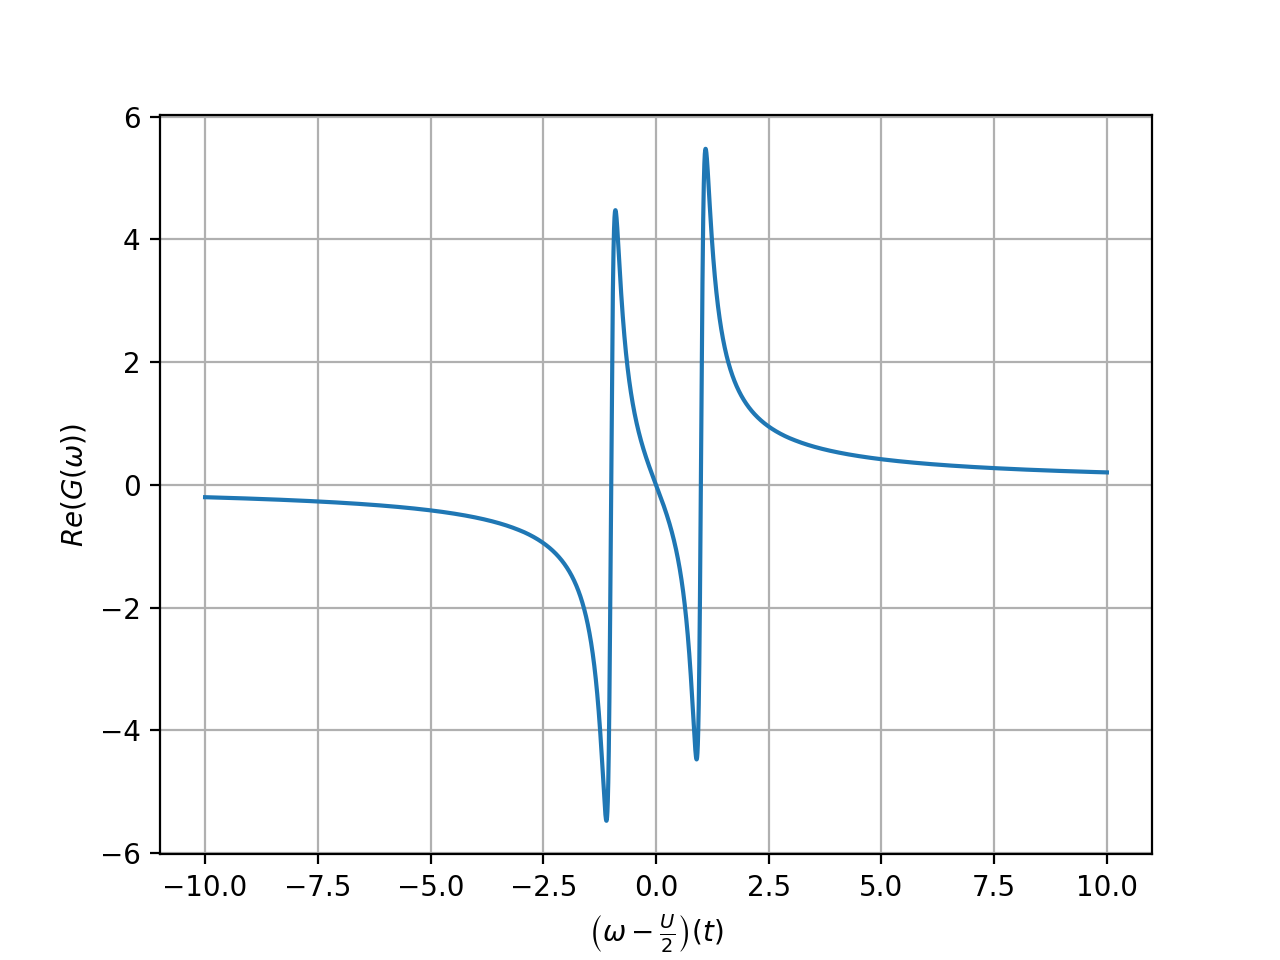
\includegraphics[max width=0.49\linewidth]{lanczosHubbard2U0Real.png}
        \end{center}
    \end{figure}
\end{frame}
\begin{frame}
    \begin{figure}
        \begin{center}
            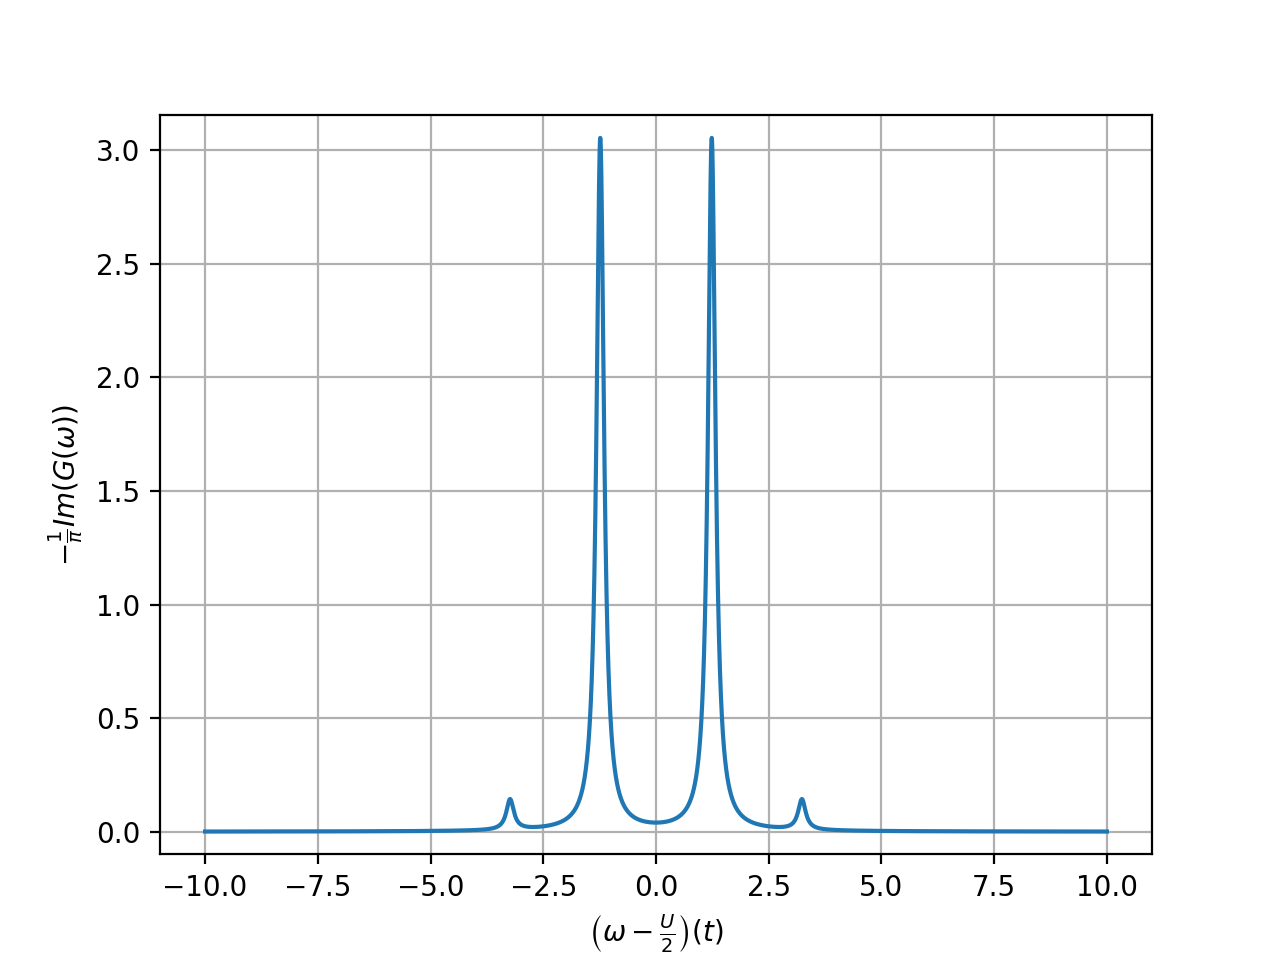
\includegraphics[max width=0.49\linewidth]{lanczosHubbard2U2Imag.png}
            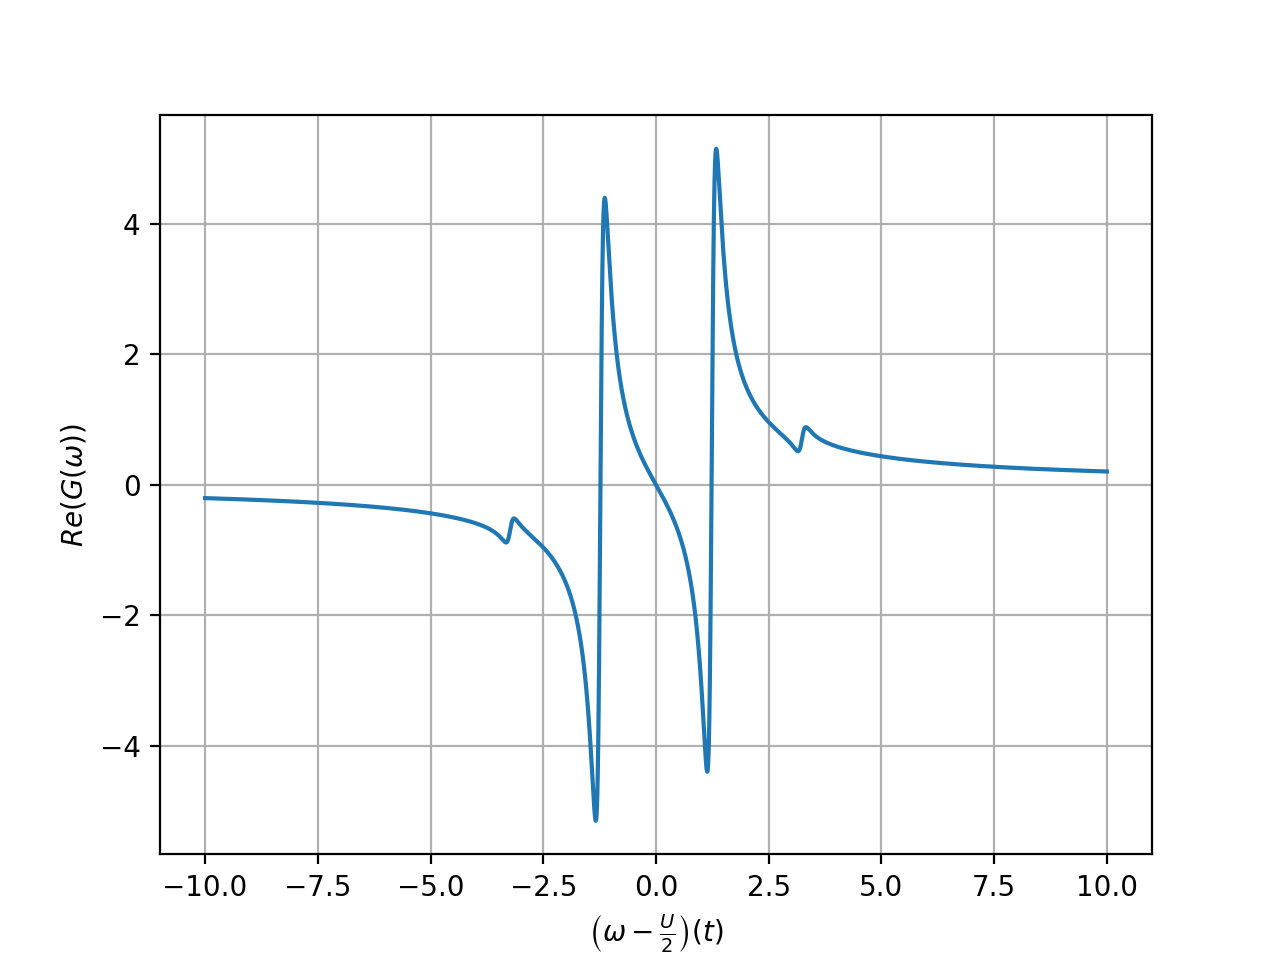
\includegraphics[max width=0.49\linewidth]{lanczosHubbard2U2Real.png}
        \end{center}
    \end{figure}
\end{frame}
\begin{frame}
    \begin{figure}
        \begin{center}
            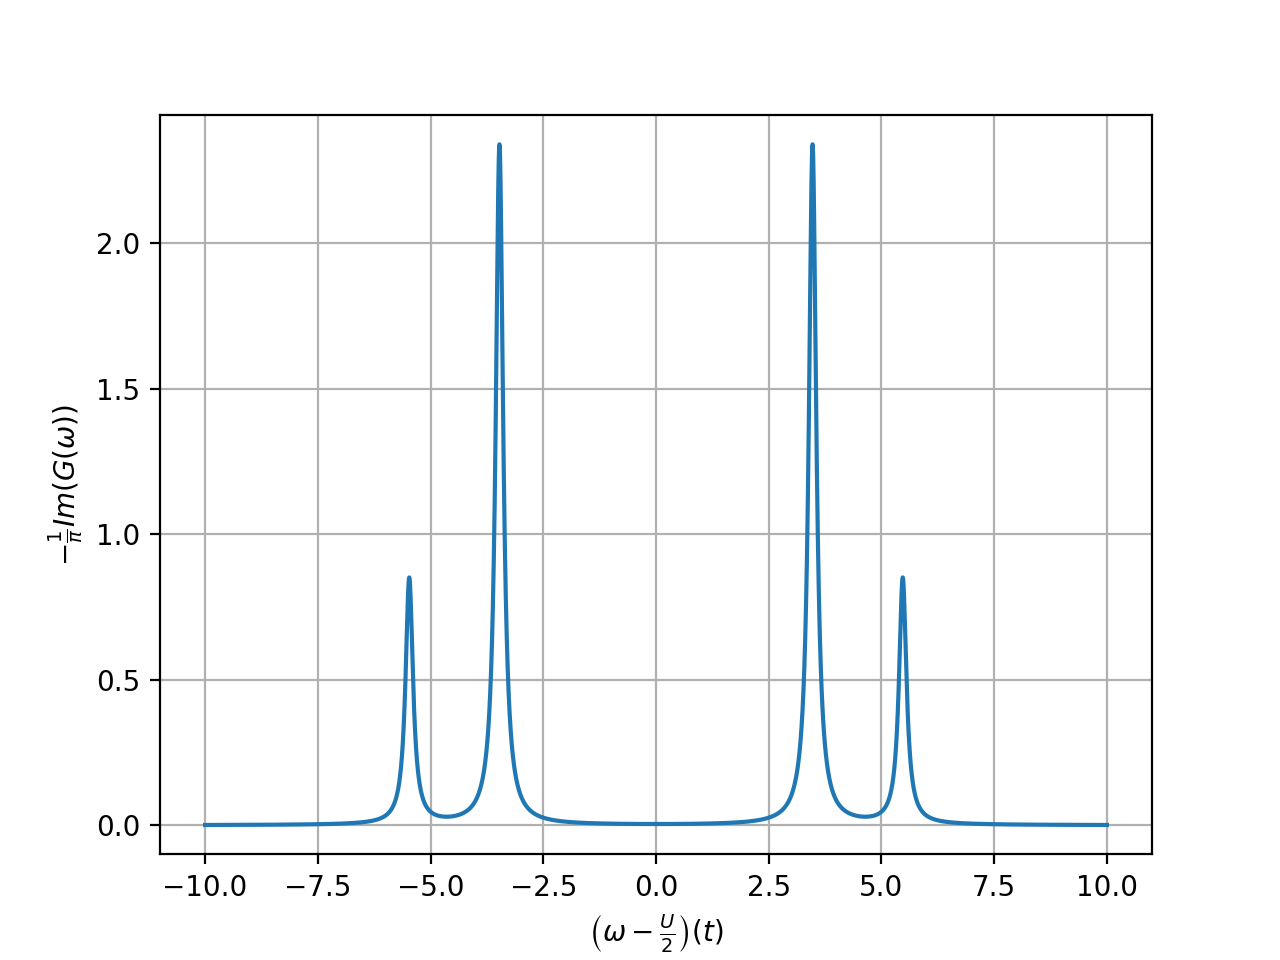
\includegraphics[max width=0.49\linewidth]{lanczosHubbard2U8Imag.png}
            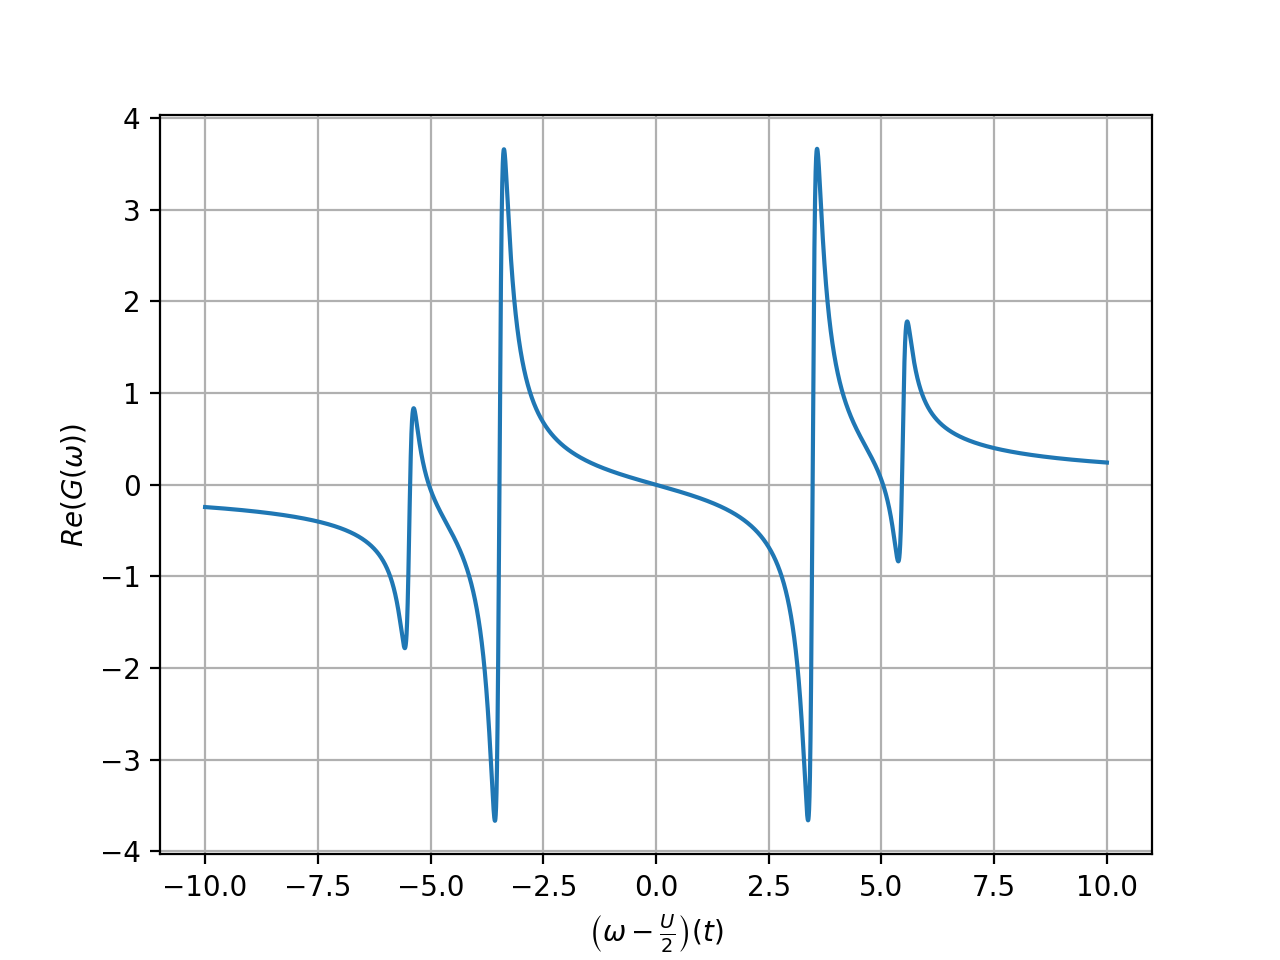
\includegraphics[max width=0.49\linewidth]{lanczosHubbard2U8Real.png}
        \end{center}
    \end{figure}
\end{frame}
\begin{frame}
    Al considerar las interacciones electrón-electrón cambian las propiedades del sistema respecto a como era en el modelo de tight-binding. Abriéndose un gran gap, de longitud $\frac{U}{2}$, en torno a la energía de Fermi.
    \begin{block}{Cambio de propiedades}
        La apertura de este gap implica un cambio de propiedades:
        \begin{itemize}
            \item \textit{Aparecen dos bandas}. El sistema, que sin interacción sólo formaba una banda, ahora pasa a formar dos bandas muy definidas, apareciendo un gap de energías prohibidas muy claro.
            \item \textit{Perdemos la conductividad.} Ahora, la banda inferior está totalmente llena, y el gap es tan grande que los electrones no pueden saltar fácilmente de una a otra banda (el término de hopping resulta insuficiente para hacerlos saltar). De este modo, hemos encontrado que nuestro material pasa a ser un aislante al introducir una interacción.
        \end{itemize}
    \end{block}
    En resumen, un material, que en un modelo tight-binding conduciría la electricidad, al considerar una interacción entre electrones repulsiva, pierde esta conductividad. Notemos que en este caso, el modelo de Hubbard modeliza la repulsión electrónica.
\end{frame}
\begin{frame}{Desarrollo - Superconductividad}
    En general, en el caso anterior, teníamos un estado fundamental en el que no se formaban pares electrón-electrón. El gran gap que se abría, impedía la conductividad en el material.
    $$
    \begin{array}{ccc}
        |\uparrow, \downarrow, \downarrow, \uparrow, \downarrow, \uparrow\rangle & |\uparrow, \uparrow, \uparrow, \downarrow, \downarrow, \downarrow\rangle & |\uparrow, \uparrow, \downarrow, \downarrow, \uparrow, \downarrow\rangle
    \end{array}
    $$
    Ahora vamos a modelizar una interacción atractiva. Esto podría representar las interacciones electrón-fonón, que darán lugar a un estado fundamental con pares. Son de la forma:
    $$
    \begin{array}{ccc}
        |\uparrow\downarrow, 0, 0, \uparrow\downarrow, 0, \uparrow\downarrow\rangle & |\uparrow\downarrow, \uparrow\downarrow, \uparrow\downarrow, 0, 0, 0\rangle & |\uparrow\downarrow, \uparrow\downarrow, 0, 0, \uparrow\downarrow, 0\rangle
    \end{array}
    $$
    Estos pares no son pares de Cooper, puesto que falta las interacciones con la red para poder considerarlos. Pero son algo parecido, que podemos tratar como una señal de portadores de superconductividad.
\end{frame}
\begin{frame}
    A continuación, representamos el número promedio de pares en función de $U$ y de $t$.
    \begin{equation}
        P = \sum_i\langle\psi_0|c_{i\downarrow}^{\dagger}c_{i\uparrow}^{\dagger}c_{i\uparrow}c_{i\downarrow}|\psi_0\rangle
    \end{equation}
    \begin{figure}
        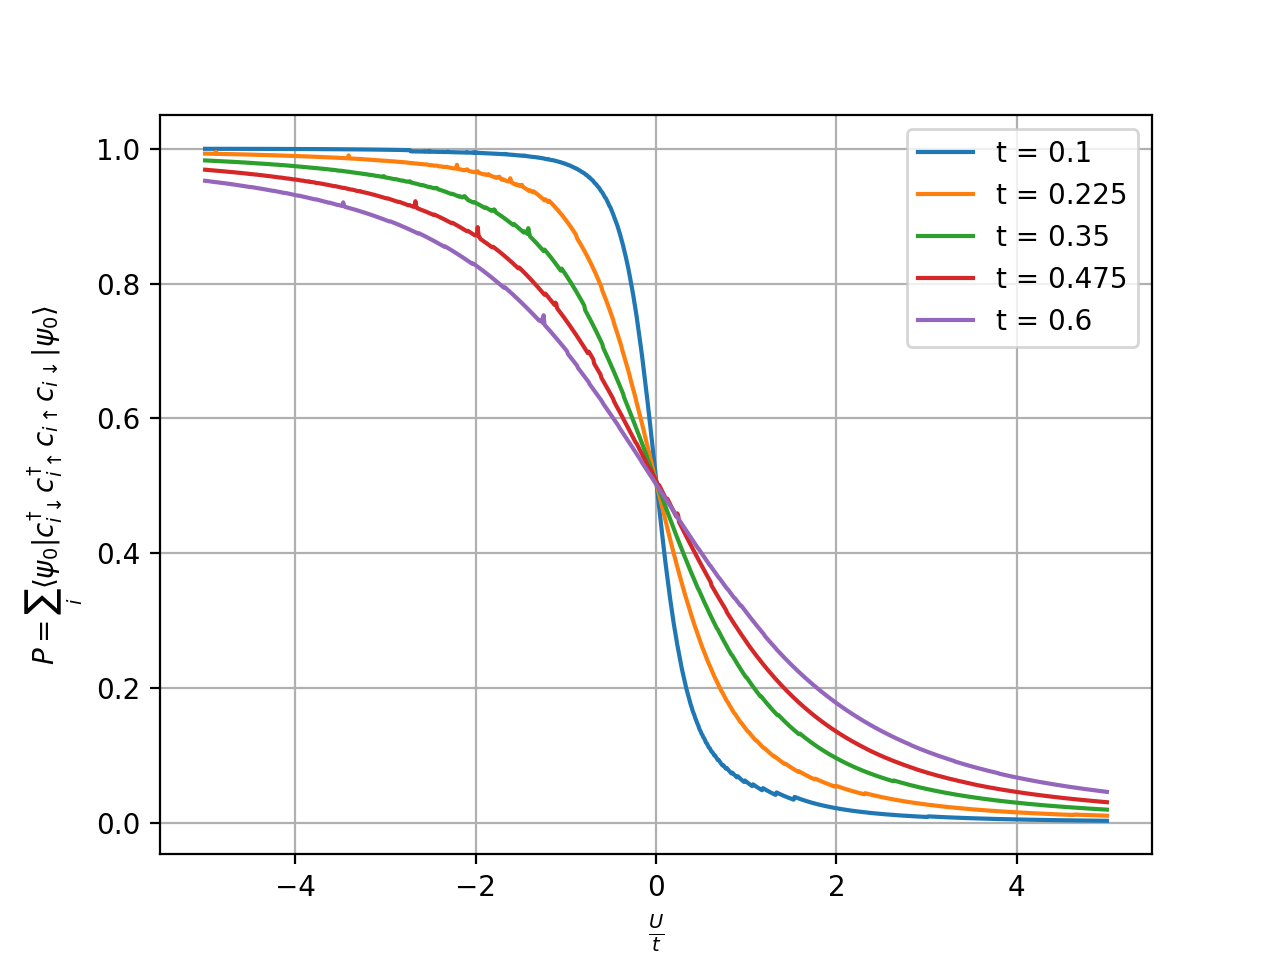
\includegraphics[max width=0.7\linewidth]{ProbabilityPairsAll.png}
    \end{figure}
\end{frame}
\begin{frame}{Desarrollo - Tiempos de cálculo}
    \subsection{Tiempos de cálculo}
    \begin{figure}
        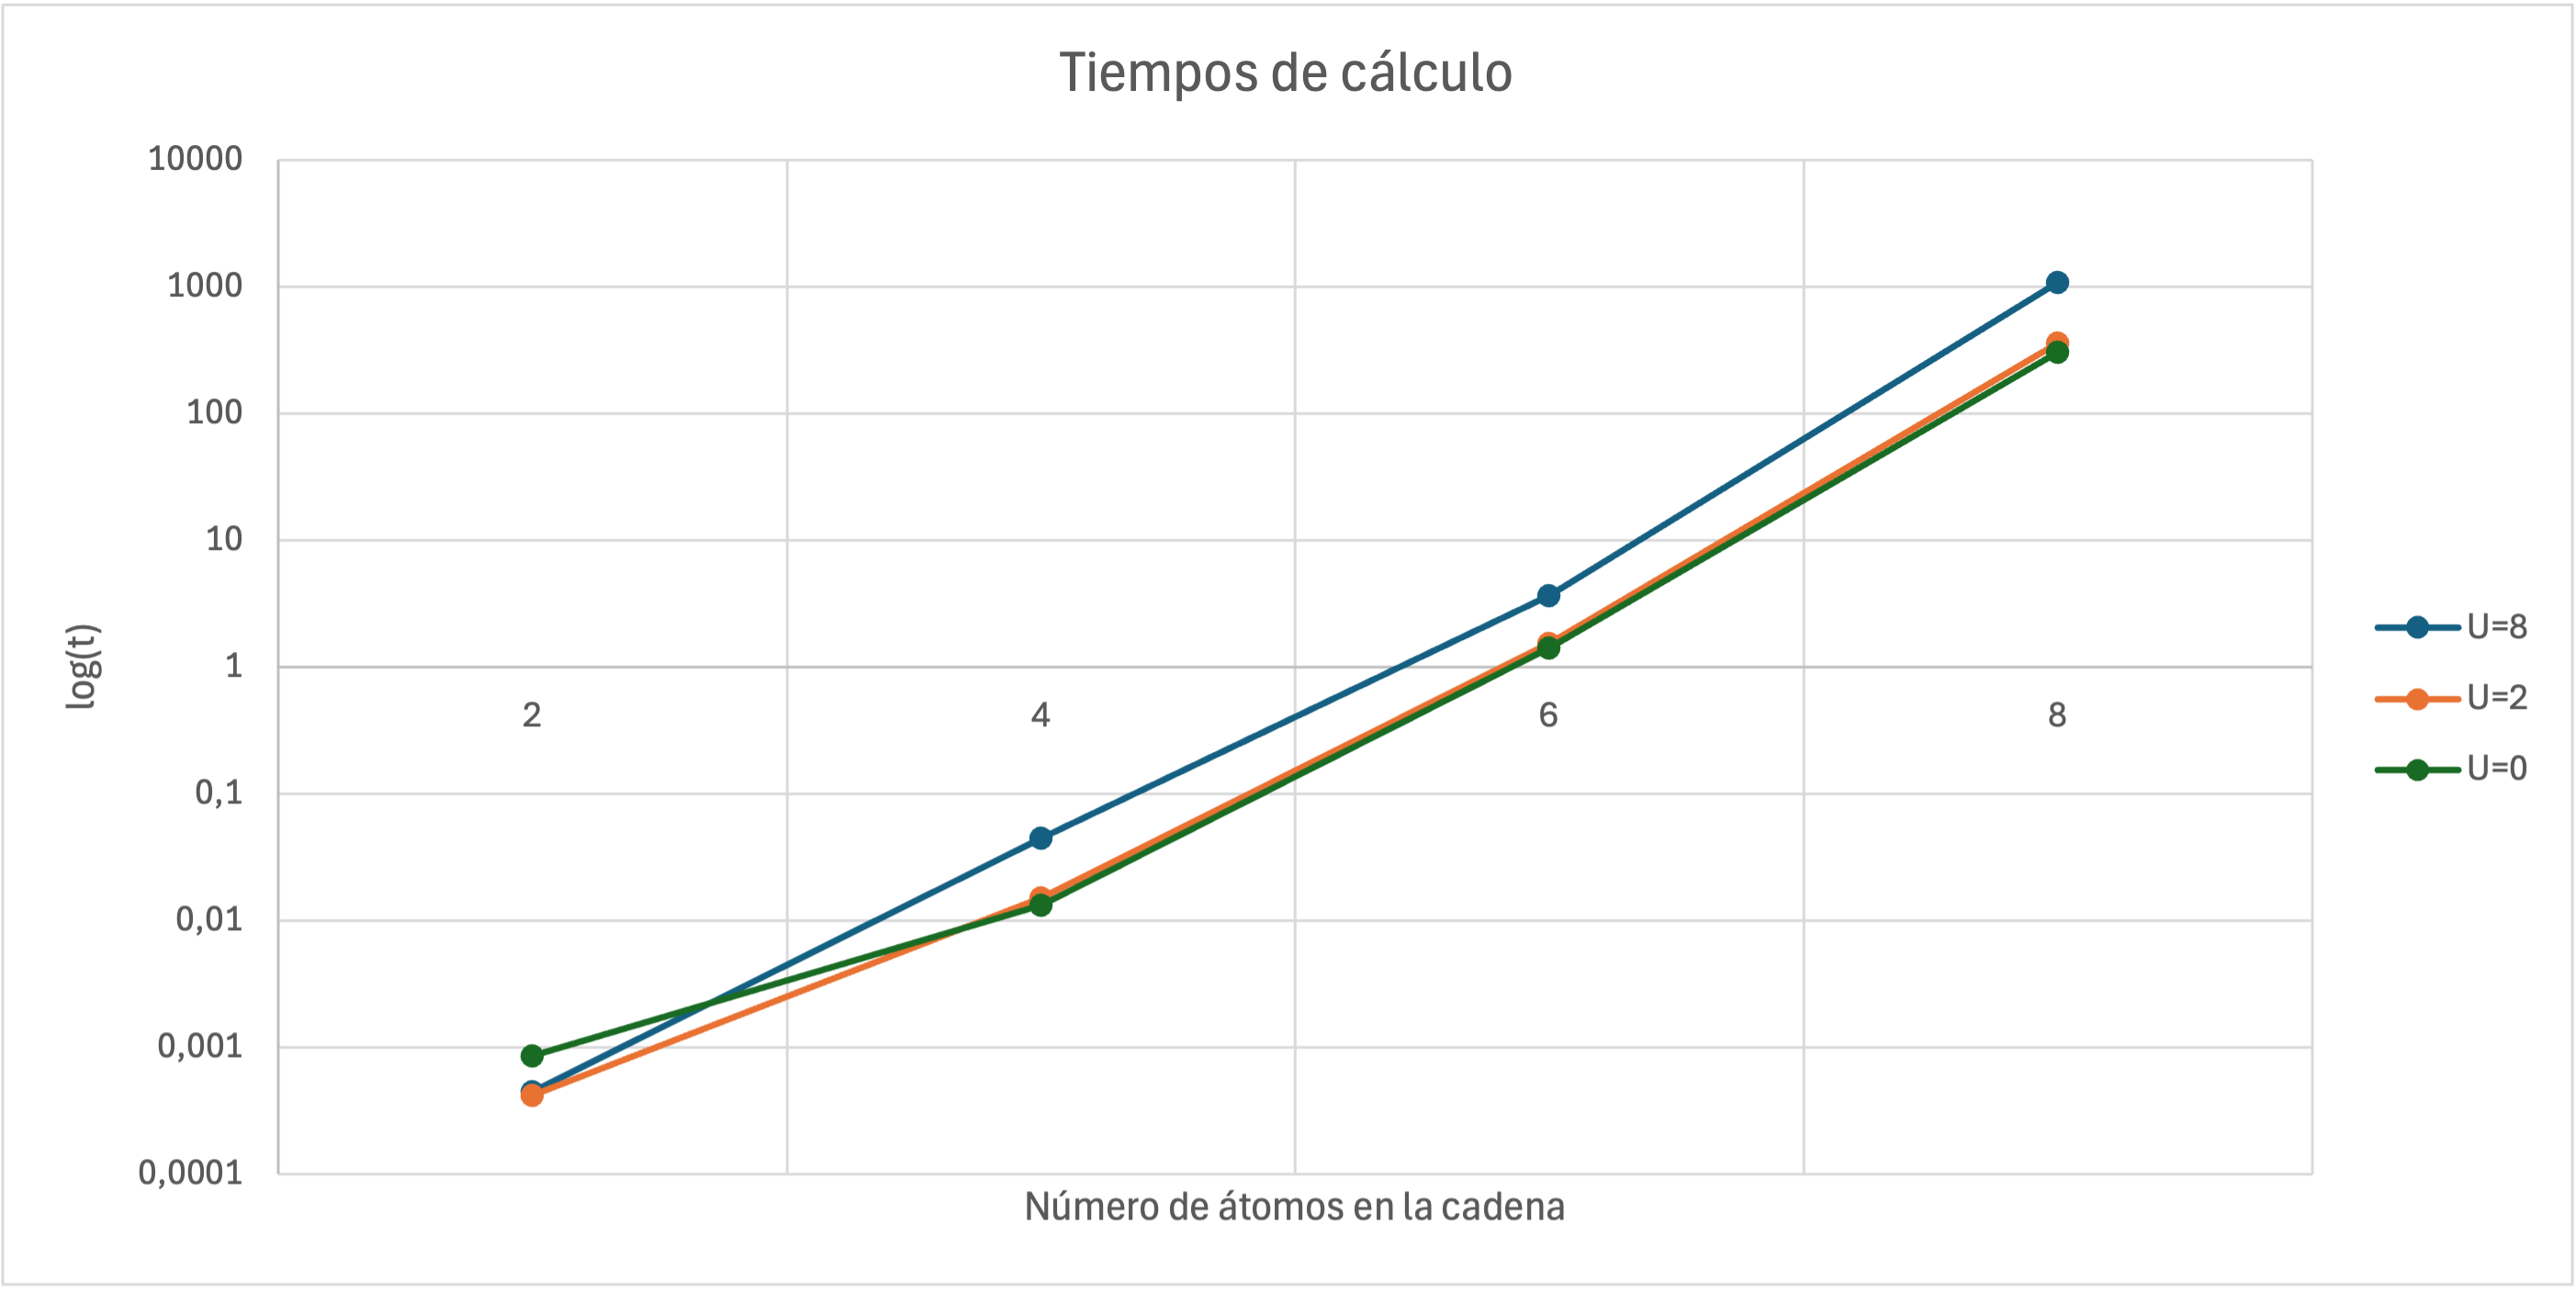
\includegraphics[max width=0.75\linewidth]{tCalcs.png}
    \end{figure}
    \begin{block}{Complejidad de cálculo}
        Si representamos el tiempo de cálculo en escala logarítmica, frente al número de átomos, podemos estimar que la complejidad del cálculo crece como $\mathcal{O}(10^N)$.
    \end{block}
\end{frame}
\begin{frame}
    \begin{figure}
        \begin{center}
            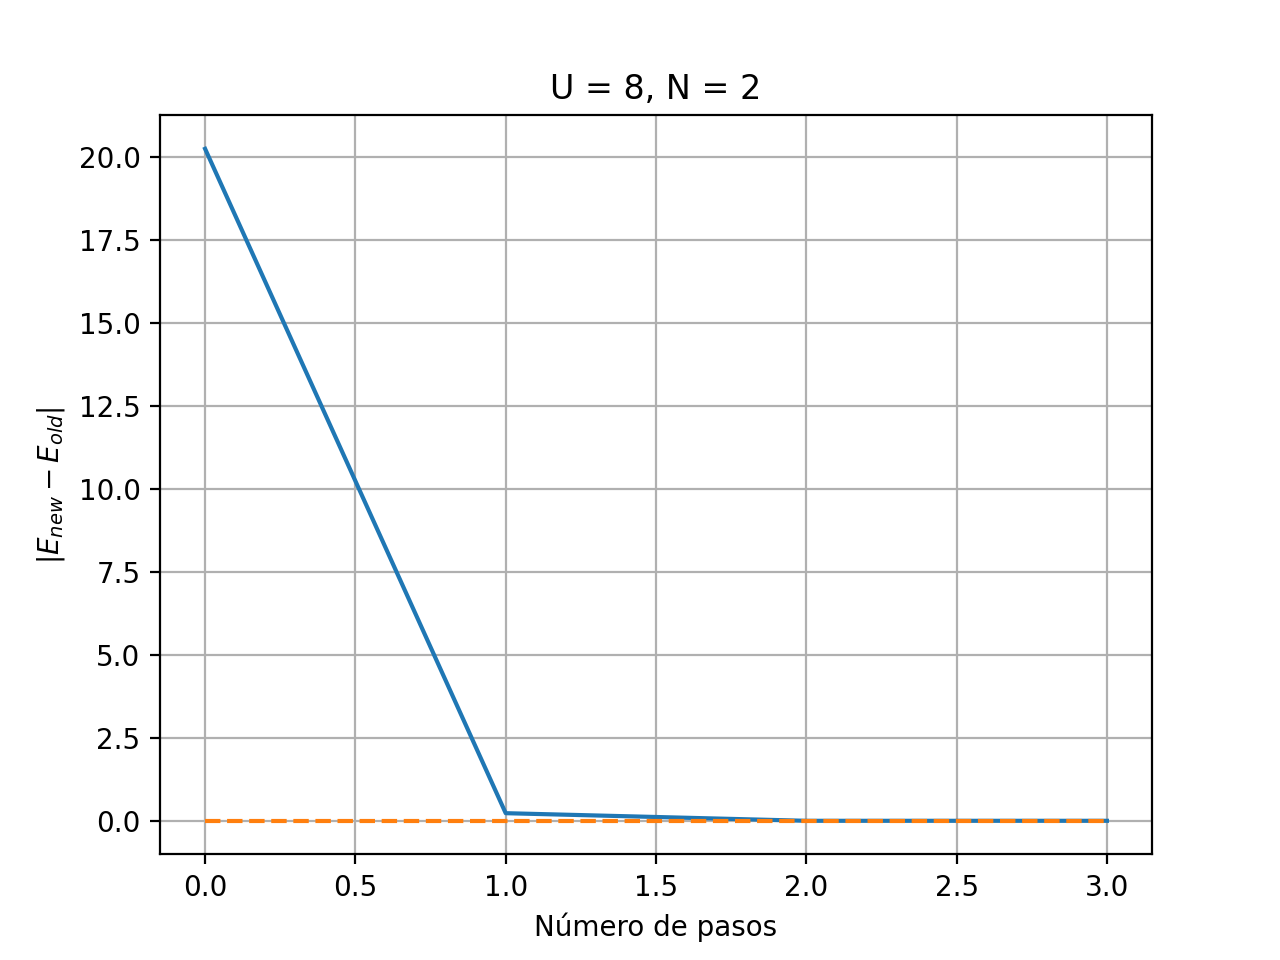
\includegraphics[max width=0.45\linewidth]{convergenceU8N2.png}
            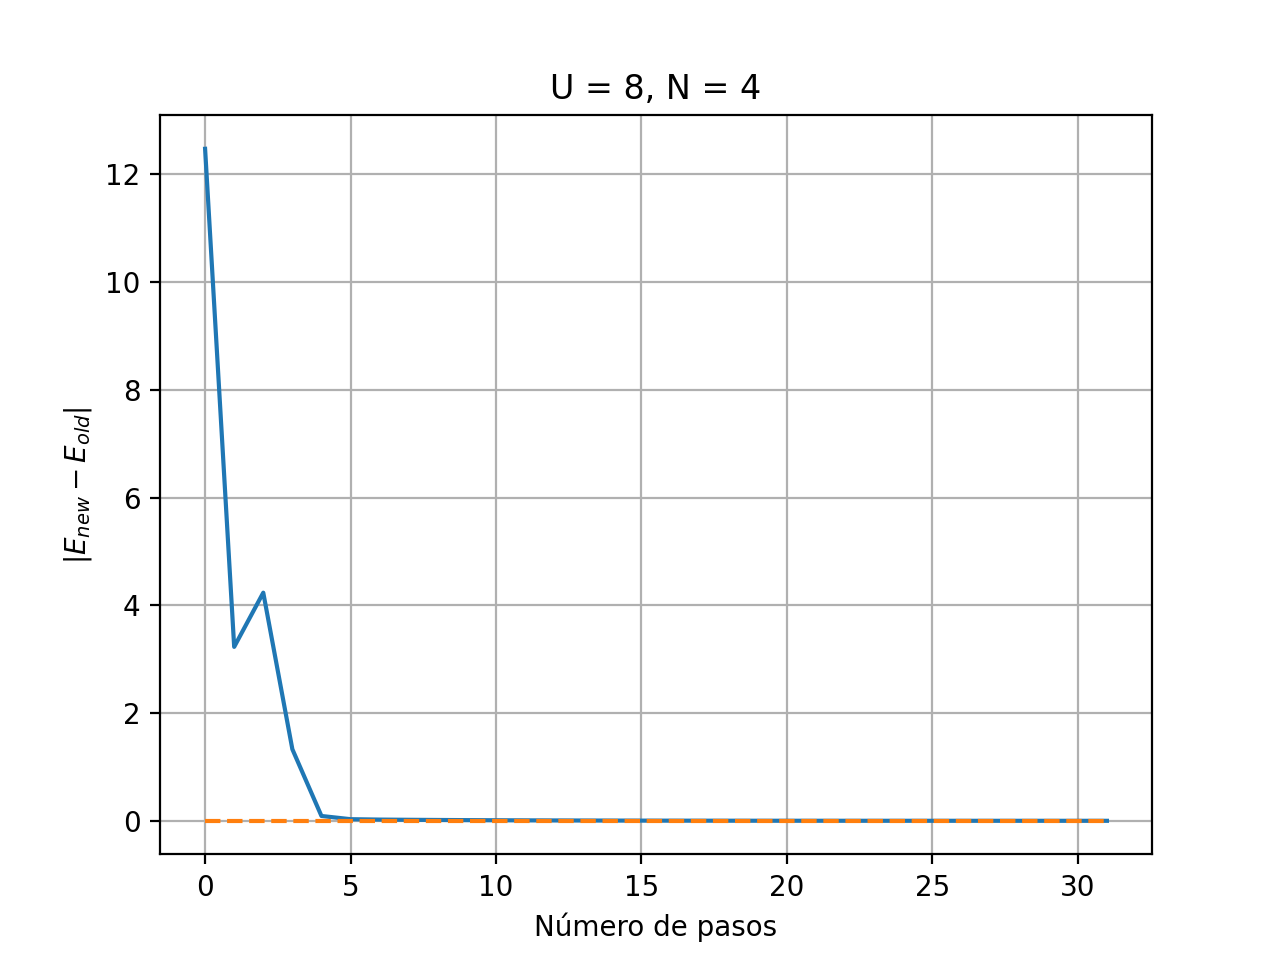
\includegraphics[max width=0.45\linewidth]{convergenceU8N4.png}
            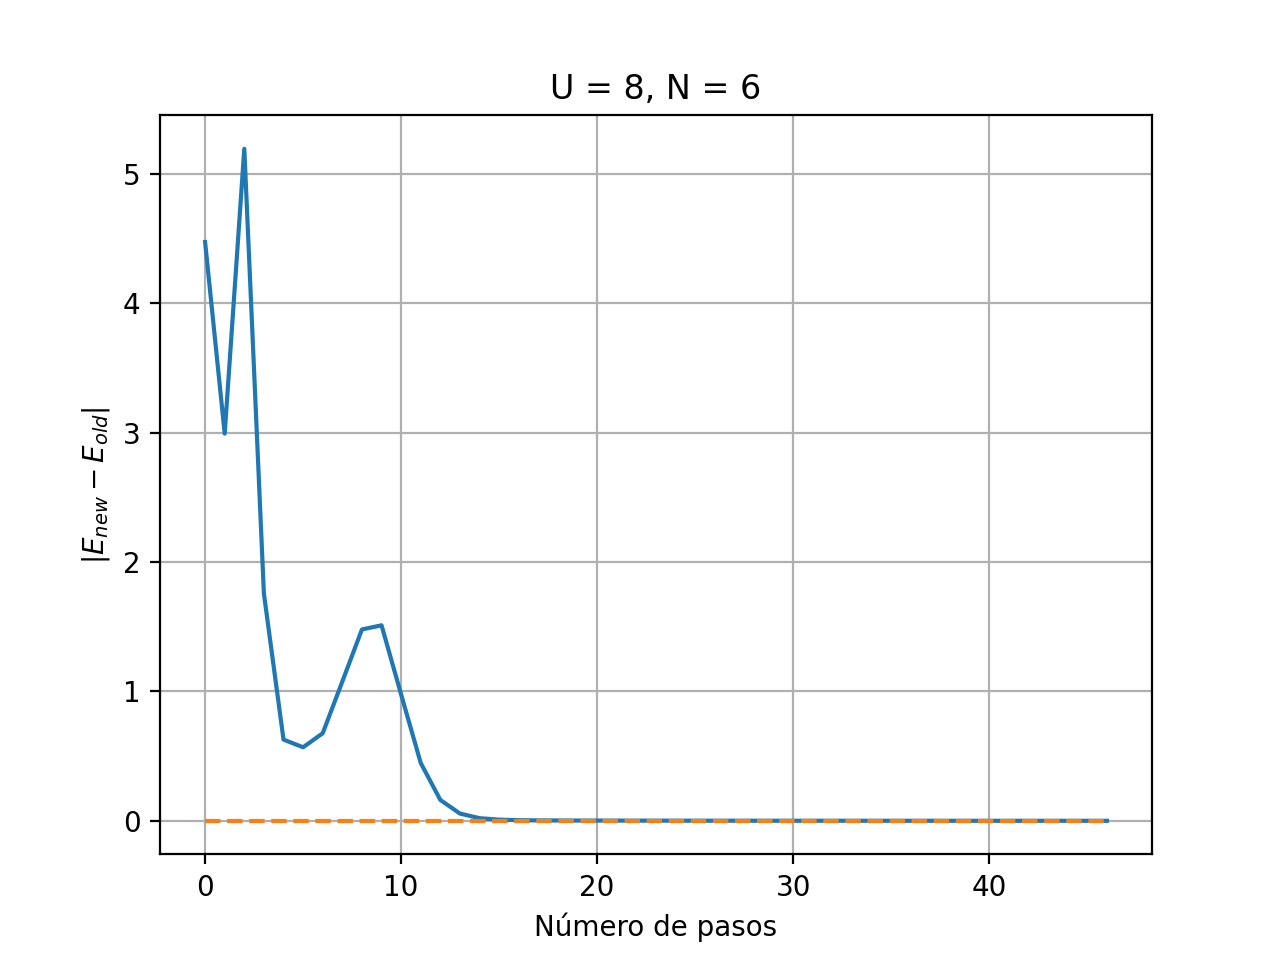
\includegraphics[max width=0.45\linewidth]{convergenceU8N6.png}
            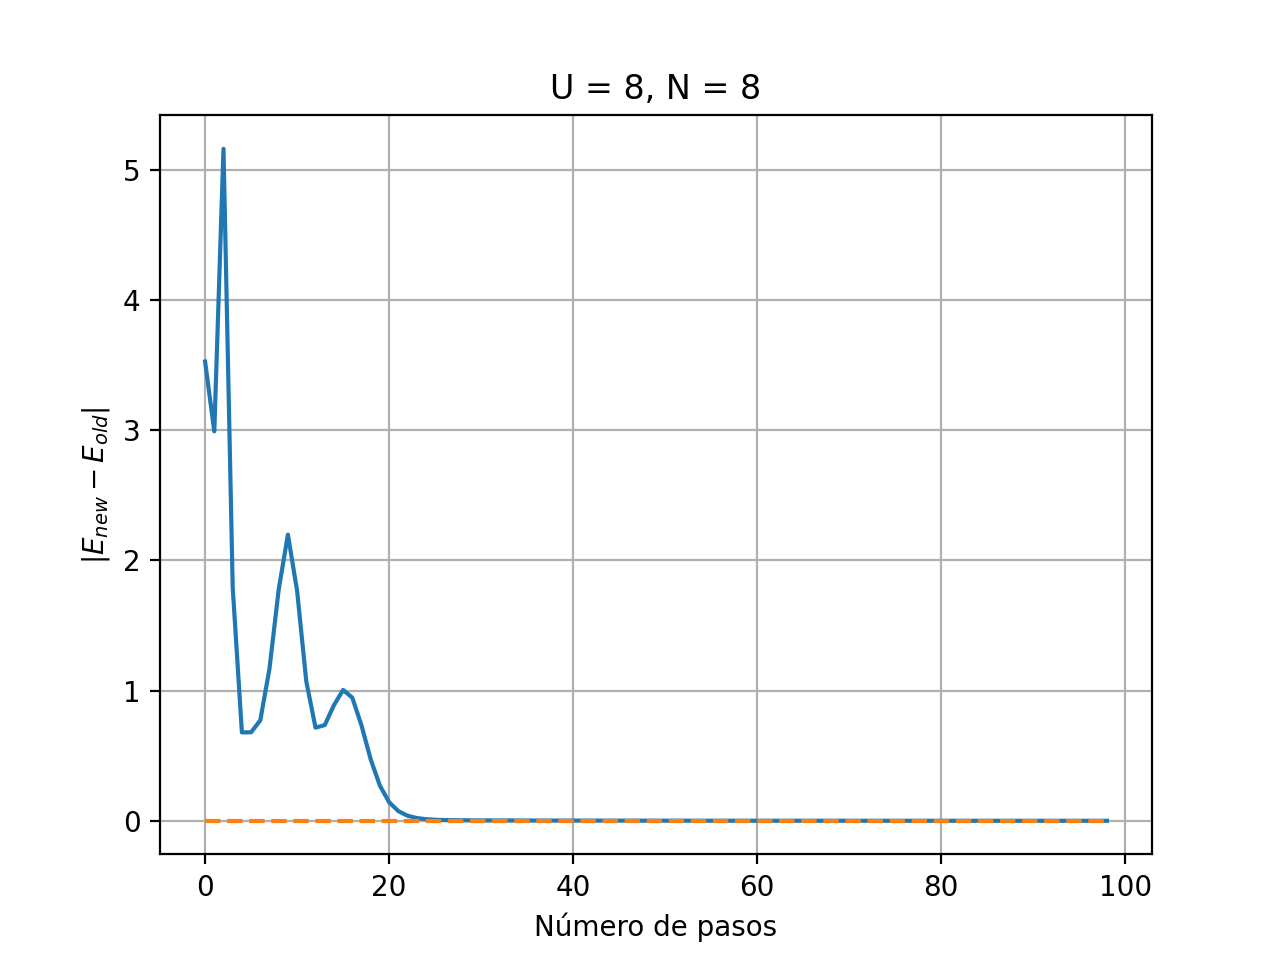
\includegraphics[max width=0.45\linewidth]{convergenceU8N8.png}
        \end{center}
        \label{fig:convergenceBad}
    \end{figure}
\end{frame}
\begin{frame}{Conclusiones}
    \section{Conclusiones}
    \begin{block}{Conclusiones}
        \begin{itemize}
            \item El modelo de Hubbard permite modelizar interacciones sencillas entre electrones.
            \item El método de Lanczos es un método potente, pero con un coste computacional bastante elevado para este problema.
            \item Las interacciones entre electrones causan una desviación respecto al modelo de tight-binding, que causan una pérdida de la conductividad respecto al mismo.
            \item Si consideramos una interacción atractiva, aparecen pares que parecen conducir la superconductividad, además están protegidos frente a defectos por la fuerza de $U$. Sin embargo, se requiere de una descripción más detallada.
        \end{itemize}
    \end{block}
    En simulaciones DFT, se incluye el término de Hubbard para evitar predecir conductividad en materiales que no lo son.
\end{frame}
\begin{frame}[allowframebreaks]{Referencias}
    \section{Referencias}
    \printbibliography
\end{frame}
\end{document}